%=========================================================================
% Autor: Sergey Panov
\chapter{Úvod}
V dnešní době existuje velké množství informací uložených v různých podobách: text, video, infografika, zvuky a další. Kvůli objemům těchto dat, které ročně přibývají, je výzkum v~oblasti vyhledávání a vývoje pokročilých nástrojů pro vyhledávání zcela zásadní. 

Tato práce se věnuje zkoumání problematiky vyhledávání v rozsáhlých textových korpusech. Výzkum problematiky vyhledávání v textových zdrojích je aktuální téma, protože nejvíce informací na Internetu je uložených v textovém formátu a při vyhledávání v těchto informacích se používají textové dotazy. Například, největší webový vyhledávač Google denně provádí $3.5$ miliardy vyhledávání\footnote{\href{http://www.internetlivestats.com/google-search-statistics/}{http://www.internetlivestats.com/google-search-statistics/}}. Avšak Google není jediným webovým vyhledávačem, existuje i řada dalších, světově známých vyhledávačů, jako Yahoo, Bing apod.  Existuje také velké množství lokálně známých vyhledávačů jako Seznam, Yandex či DuckDuckGo. Další vyhledávací nástroje jsou používané v rámci organizací\,(knihovny, univerzity, společnosti), které provádějí vyhledávaní v lokálních úložištích.

Tato práce vznikla v rámci školní výzkumné skupiny znalostních technologií\,(KnoT), která se věnuje výzkumu v oblasti interakce člověka s počítačem a zaměřuje se na praktické aplikace zpracování přirozeného jazyka.

V rámci této práce pokračuje vývoj systému, který je schopen stáhnout a zpracovat určitý zdroj dat. Systém se skládá z více programů. Tato práce se věnuje návrhu a vývoji vyhledávací části, která by měla být schopna provádět vyhledávání v rozsáhlých textových korpusech, a aplikaci schopné komunikovat s vyhledávací částí.

Ve \ref{chapter2} kapitole věnované indexování sémanticky obohacených textů se rozebírají základní pojmy, které jsou zcela zásadní pro pochopení tématu. Náplní kapitoly je teorie popisující vyhledávaní v textových korpusech a přístupy, které se používají pro zvýšení přesnosti a~zrychlení vyhledávaní. 

Vzhledem k tomu, že práce je pokračováním jíž existujícího projektu, je nutné mít představu o tom, co všechno projekt obsahuje.  Kapitola \ref{chapter3}  stručně popisuje jednotlivé programy, vyvinuté v rámci celého projektu.

Uživatelé  interagují s vyhledávacími systémy prostřednictvím požadavků. Kapitola \ref{chapter4}~se věnuje popisu dotazování bez znalosti struktury uložených dat a uvádí příklady reálně existujících systémů.  Také jsou zde popsáné úkoly, které mají být splněny v této práci.


Kapitola \ref{chapter5} dále zkoumá požadavky kladené na systém a na základě těchto požadavků navrhuje jednotlivé části, které plní definované úkoly. 
 
Na to navazuje kapitola \ref{chapter6}, která pojednává o implementaci navržených částí. 

Při vývoji softwaru je důležitá etapa testování a experimentování s vyvinutým produktem. Kapitola \ref{chapter7} se věnuje definici metrik, které jsou důležité pro tuto práci, a popisuje průběh fází testování a experimentování se systémem s následnou analýzou získaných výsledků.


Závěrečná kapitola \ref{chapter8} shrnuje dosažené výsledky této práce a poukazuje na možnosti rozšíření funkcionality systému. 

\chapter{Indexování sémanticky obohacených textů}
\label{chapter2}

Hlavními cíli této kapitoly je seznámení s pojmem \uv{sémanticky obohacené texty}, s přístupy pro práci s obohacenými texty a reprezentací sémanticky obohacených textů. Postupně se vysvětlují základní pojmy potřebné pro lepší pochopení práce. Jsou zde také popsány rozdíly při vyhledávaní v prostých a strukturovaných textech, jaké prvky můžou plnit role indexů, k čemu se používají indexy při vyhledávaní ve strukturovaných textech a co vlastně je \uv{anotace}. V této části jsou také probrány základní třídy modelů pro vyhledávání ve~strukturovaných textech a uvedeny konkretní příklady přístupů, které vycházejí z těchto modelů. 

Po seznámení s modely tato práce pojednává o  reprezentaci sémantických dat a o způsobech vytváření sémanticky obohacených dat. Na konci kapitoly je popsána architektura  systémů pracujících s obohacenými texty.   

\section{Základní pojmy}
Nejprve je potřeba se seznámit se základními pojmy, které jsou v této práci často používané. Tato část se věnuje právě vysvětlování základních pojmů. Postupně se zde rozebírají pojmy jako \textbf{token}, \textbf{strukturovaný text} a \textbf{index}  v kontextu, ve kterém se používají v této práci.

\subsection*{Token}

Nejprve si definujeme pojem \textbf{token}. Tento pojem se široce používá v odborných textech v anglickém jazyce a v závislosti na kontextu může nabývat různých významů. V rámci této práce pod pojmem \textbf{token} rozumíme posloupnost nebílých znaků\,(pismena, čísla, interpunkční znaménka apod.). V textu se tokeny oddělují bílými znaky\,(mezera, tabulátor apod.).    

\subsection*{Strukturovaný text}
\label{structuredText}
\textbf{Strukturovaný text} je text, zapsaný podle schématu, ve kterém se označují klíčové prvky. Klíčovou je právě existence schématu, na základě kterého je text formátován.

 Na vyšší úrovní abstrakce můžeme na strukturovaný text nahlížet jako na strukturovaná data.  \textbf{Strukturována data} jsou definovaná jako libovolná množina hodnot, která odpovídá určitému schématu nebo typu \cite{Arasu:2003:ESD:872757.872799}. Rekurzivně je \emph{typ} definován následovně:
\begin{itemize}
\item \emph{Základní typ\,(Basic type)} $B$ je množina primitivních prvků, ze které se skládají složitější typy.

\item Když $T_1, \ldots, T_n$ jsou typy, pak uspořádaný seznam $\langle\,T_1, \ldots, T_n\,\rangle$ je také typ. Typu $\langle\,T_1, \ldots, T_n\,\rangle$ se říká \emph{zkonstruovaný typ} z typů $T_1, \ldots, T_n$ s použitím konstruktoru uspořádaného seznamu.

\item Když typ $T$ je typem, pak $\{T\}$ je také typem. Typu $\{T\}$ se říká  \emph{zkonstruovaný typ} z~$T$ s použitím konstruktoru množiny. 
\end{itemize}
Pojem \emph{instance} schématu je rekurzivně definován jako:
\begin{itemize}
\item Instance základního typu $B$ je libovolná řada primitivních prvků.

\item Instance typu  $\langle\,T_1, T_2, \ldots, T_n\,\rangle$ je uspořádaný seznam $\langle i_1, i_2, \ldots, i_n \rangle$ kde $i_1, i_2, \ldots, i_n $ jsou instancemi typů $T_1, T_2, \ldots, T_n$. Instance $i_1, i_2, \ldots, i_n$ jsou atributy uspořádaného seznamu.

\item Instance typu $\{T\}$ je množinou elementů $\{e_1, e_2, \ldots, e_n\}$, kde $e_i\,\left(1 \leq i \leq n\right)$ je instance typu $T$. 
\end{itemize}

Jako synonymum termínu \emph{instance} se používá termín \emph{hodnota}. Příkladem může být struktura webových stránek, které obsahují informace o knihách. Na každé stránce je uveden název, seznam autorů a cena knihy,  každý autor má uvedené jméno a příjmení. Na základě výše uvedených rekurzivních definic můžeme popsat strukturu stránek jako $S_1 = \langle B, \{\langle B, B \rangle_{T_3}\}_{T_2}, B\rangle_{T_1}$. Schéma se skládá ze dvou konstruktorů uspořádaného seznamu $T_1$ a $T_3$ a jednoho konstruktoru množiny $T_2$. Instancí schématu je hodnota $x_1 = \langle t, \{\langle f_1, l_1 \rangle, \langle f_2, l_2 \rangle \}, c\rangle$, kde $t$ reprezentuje název, $\langle t_n, l_n \rangle$ jméno a příjmení, $c$ cenu.


\subsection*{Index}
S pojmem \textbf{index} se setkáváme v různých kontextech: index databáze, index cen výrobců, index lomu atd., s ohledem na množství kontextů, ve kterých se tento pojem používá, je zapotřebí dát mu definici, kterou budeme uvažovat v této práci.

Podle \emph{National Information Standards Organization\,(NISO)}  je \textbf{index}  jakýmsi návodem navrženým pro identifikaci témat nebo  rysů dokumentů s cílem zajistit vyhledání dokumentu nebo části dokumentu \cite{GuidlinesForIndexesAndRelated}. 

Podle Oxfordského slovníku angličtiny\footnote{\href{https://en.oxforddictionaries.com/definition/index}{https://en.oxforddictionaries.com/definition/index}} je \textbf{index} abecední seznam jmen, subjektů apod., s odkazem na stránky, na kterých byly zmíněny.

Existují i další definice pojmu \emph{index}, ale všechny  vyjadřují společnou myšlenku\,--\,\textbf{index} je strukturou dovolující zrychlený přístup k určité informaci\,(například článku) bez nutnosti analýzy celého zdroje informací\,(například knihy) \cite{IndexingBooks}. Uživatel se obrátí na index v případě potřeby rychlého přístupu k nějaké specifické informaci. V případě, že informace neodpovídá očekávané, lze usoudit, že index nesplňuje svůj primární účel.



\section{Pokročilé vyhledávání v prostých a strukturovaných textech}

V této části jsou vysvětleny hlavní rozdíly mezi vyhledáváním ve strukturovaných a v nestrukturovaných textech. Také jsou zde popsány třídy, do kterých spadají různé modely pro vyhledávání ve strukturovaných textech.


\subsection{Rozdíly přístupů pří vyhledávání ve strukturovaných a nestrukturovaných textech}

Nejprve definujeme cíl vyhledávání v textu. Intuitivně je jasné, že hlavním cílem při vyhledávání v textu\,(strukturovaném nebo nestrukturovaném) je určení výskytů fragmentů odpovídajících vyhledávacímu dotazu. Pro vyhledávání v nestrukturovaných textech se používá princip \emph{shody řetězců\,(string matching)}, což směruje k použití algoritmů jako Rabinův-Karpův algoritmus, algoritmus Boyear–Moora apod. \cite{books/daglib/0029345}.  Jádrem tohoto přístupu je vyhledávání vzorků v textu. Existují také různé modifikace tohoto přístupu, jako například vyhledávání klíčových slov \cite{TEXT_ANALYZER}, vyhledávaní shodných slov apod. 

Při vyhledávání ve strukturovaném dokumentu se očekává existence polí\,(fields) nebo značek, vytvořených autorem nebo automaticky, jejichž obsah se používá pro tvorbu indexů, které přispívají k zrychlení vyhledávání v textu. Zpravidla dotazy, které se používají pro vyhledávání ve strukturovaných textech, používají různé kombinace podmínek,  určujících pole a hodnoty polí \cite{Zhao:2009:EES:1645953.1646175} \cite{Luo:2012:ITR:2900728.2900821}.

\subsection{Modely vyhledávání ve strukturovaných textech}

Modely vyhledávání poskytují možnost formálního dotazování nad strukturovanými texty. Jak již víme, strukturovaný dokument se skládá z vlastního textu a struktury, která odpovídá určitým kritériím. Jedním z nejpopulárnějších způsobu reprezentace strukturovaných textů je značkovací jazyk XML, ve kterém elementy XML určují strukturu textu. Ideálně by se modely pro vyhledávání  měly skládat ze třech částí: 
\begin{enumerate}
\item model textu,
\item model struktury,
\item model jazyka.
\end{enumerate}
Model textu definuje rozdělení textu na tokeny a\,(nebo) na jiné prvky jako lemmata apod. Model struktury definuje části textu. Nepřerušovaným sousedícím prvkům textu se typicky říká  \emph{regiony} nebo \emph{segmenty}\,(např. věty, odstavce), které se skládají z tokenů.  Model jazyka definuje množinu operátorů nad textem, které dovolují vytvářet různé dotazy \cite{STRUCTURED_TEXT_RETRIEVAL_MODELS}.

V poslední době bylo vyvinuto množství modelů. Zde si ukážeme několik obecných tříd, do kterých spadají různé modely. Základem následujícího výkladu je článek pánů H. Meusse a C.~M.~Stronhmaiera \cite{meuss1999improving}. Modely spadající do těchto tříd nahlížejí na strukturovaný dokument jako na orientovaný graf\,(zpravidla strom). Uzly obsahují text jednotlivých segmentů. Vztahy mezi elementy struktury jsou reprezentovaný prostřednictvím hran. Uzly obsahující jiné uzly\,(kapitola má více podkapitol) se sdružují do svazů. Vyhodnocení dotazu se provádí pomocí různých struktur:
\begin{enumerate}
\item \emph{Index textu}: implementuje mapovaní tokenů z dotazu na tokeny v regionech\,(ve větách, odstavcích).

\item \emph{Index struktury}: implementuje mapovaní elementů struktury z dotazu na elementy struktury v dokumentu.
\end{enumerate}


Při vysvětlení principů činnosti modelů z jednotlivých tříd použijeme dotaz pro získaní množiny názvů kapitol, ve kterých je popsaný jazyk \emph{Java} \ref{javaReading}:


\begin{lstlisting}[label=javaReading, caption={Vzorový dotaz}, captionpos=b]
		    Get all titles of chapters reading Java.
\end{lstlisting}
Jednotlivé třídy modelů jsou rozděleny podle jejich strategií vyhodnocování dotazu.

\textbf{Model vyhodnocování dotazu shora dolů na základě syntaktického stromu}: Do třídy spadá větší část modelů známých z literatury, jako PAT Expressions, Overlapped Lists, Proximal Nodes \cite{baeza1996integrating}. Tyto modely vytvářejí syntaktický strom z dotazu a následně vyhodnocují jednotlivé uzly. Aplikace operátoru ze stromu se provede, až budou vyhodnoceni jeho potomci. Po vyhodnocení potomků  se provede aplikace operátoru a výsledek se zapíše do uzlu operátoru. Další vyhodnocení pokračuje směrem nahoru ke kořenu. Při vyhodnocení uzlů se používají indexy textu a struktury.

Například dotaz \ref{javaReading} se dá přepsat podle notace modelu Proximal Nodes tak, jak je uvedeno ve výpisu \ref{proximalNodesNotation}.


\begin{lstlisting}[label=proximalNodesNotation, caption={Dotaz v notaci Proximal Nodes}, captionpos=b,language=Proxnodes]
		            (title same Java) in chapter
\end{lstlisting}
Při vyhodnocení se tento dotaz převádí do tvaru syntaktického stromu na obrázku \ref{syntaxTree}.
\begin{figure}[ht]
\centering
\begin{tikzpicture}[sibling distance=10em,
  every node/.style = {align=center}]]
  \node {\textbf{in}}
    child { node {\textbf{same}} 
    	child {node {\texttt{title}}}
        child {node {\emph{Java}}}
    }
    child { node {\texttt{chapter}}};
\end{tikzpicture}
\caption{Syntaktický strom \cite{meuss1999improving}}
\label{syntaxTree}
\end{figure}

Vyhodnocení tohoto dotazu se provádí v několika krocích: Použitím indexu textu se~vybere množina regionů, ve kterých je obsažen token \emph{Java}. Stejně se vyberou množiny polí \texttt{title} a \texttt{chapter} použitím indexu struktury. Prvky množiny regionů a pole \texttt{title} se skládají do párů, každý prvek páru se ukládá do uzlu. Pak se provádí aplikace operátoru \textbf{same}. V případě úspěšné aplikace\,(v poli \texttt{title} je opravdu token \emph{Java}) uzly získávají společného rodiče\,--\,uzel \textbf{same}. Pak pokračuje aplikace operátoru \textbf{in} na uzly \texttt{chapter} a \textbf{same}. V případě úspěchu aplikace operátoru\,(kapitola opravdu obsahuje podkapitolu v názvu které se~vyskytuje token \emph{Java}), uzly zase získávají společného rodiče\,--\,uzel \textbf{in}. Postupně se operátory aplikují na všechny prvky množin. Výsledkem je množina stromů, která odpovídá dotazu.



\textbf{Model vyhodnocování dotazu shora dolů na základě stromu struktury:}
Do~této třídy spadá Indexed DAG Matching formalismus \cite{Meuss1998DagMT}, což je rozšířením formalismu Tree Matching. Vyhodnocení dotazu se provádí na základě stromu struktury dotazu, na obrázku \ref{structureTree} je vizualizace výše uvedeného dotazu.

\begin{figure}[ht]
\centering
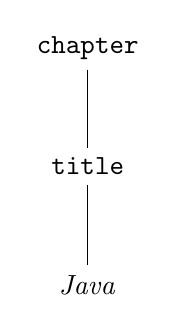
\begin{tikzpicture}[sibling distance=10em,
  every node/.style = {align=center}]]
  \node {\texttt{chapter}}
    child { node {\texttt{title}} 
    	child {node {\emph{Java}}}
    };
\end{tikzpicture}
\caption{Strom struktury \cite{meuss1999improving}}
\label{structureTree}
\end{figure}

Pro vyhodnocení dotazu se používají indexy struktury a textu, které mapují termy z~dotazu na termy stromu. Výsledkem je množina cest z dokumentů, které odpovídají stromu vytvořenému z dotazu.

\textbf{Model flexibilního vyhodnocování dotazu na základě syntaktického stromu:} Do této třídy spadá formalismus Lore systém \cite{McHugh1997LoreAD} pro dotazovaní nad grafovými strukturami dat. Jedná se o sofistikovaný mechanizmus, který pro vyhodnocení dotazu používá různé strategie\,(shora dolů, zdola nahoru, hybridní). Optimální plán vyhodnocování se určuje dynamicky na základě analýzy struktury dokumentu. Pro podporu dynamického rozhodování se používají čtyři struktury indexů. Každý index mapuje prvky z dotazu\,(termy z dotazu, vztahy nebo výrazy reprezentující cesty) na prvky dokumentu. V případě potřeby lze obohatit index o kontextovou informaci.

\section{Reprezentace a indexování sémantických dat}

Tato podkapitola vysvětluje pojem \textbf{sémanticky obohacená data} a motivaci k anotovaní dat. Popisují se zde různé druhy anotací a jejích výhody a nevýhody. Vysvětluje se pojem \textbf{znalostní báze} a její účely. Na konci podkapitoly se rozebírá reprezentace sémantických dat.

\subsection{Sémanticky obohacená data}
\label{semanticEnrichedData}
Pro lepší pochopení reprezentace sémantických dat je potřeba  seznámit se s pojmem \textbf{sémantická anotace} a vysvětlit si, k čemu slouží. Motivaci pro zavedení sémantické anotace nejlépe vysvětlují slova pana Tima Bernerse-Lee \cite{handschuh2005creating}:

\begin{quotation}
\uv{\emph{When computers not only retrieve, but also understand what data is available on the Web, we will have a new kind of Web and new types of intelligent applications in the Web. In the foreseeable future, however, machines will be too dumb to understand what people have put on the Web. Therefore, let us put computer-understandable data next to human-understandable data. Then, the computers will be smarter.}}
\end{quotation}

Tento výrok poukazuje na nezbytnost použití metadat ke zlepšení pochopení mezi počítačem\,(strojem) a člověkem. De facto jsou \textbf{anotace}  metadata přiřazena jiným datům pro rozšiřování kontextu a sémantiky; tím pádem proces \textbf{anotovaní} znamená vlastní přiřazení metadat k datům. Výsledkem procesu anotovaní je (semi)strukturovaný text. Rozlišujeme tři základní druhy anotací \cite{bechhofer2002semantics} \cite{oren2006semantic}: \emph{neformální\,(textová)}, \emph{formální\,(odkazová)} a \emph{ontologická\,(strukturováná)}.

Pod \emph{neformální anotací} si lze představit poznámku v knize. Tento typ anotace má množství problémů: například je zcela nevyhovující pro počítačové zpracování kvůli absenci struktury. Během anotovaní je také  potřeba vícekrát popisovat stejnou entitu, což zvyšuje pravděpodobnost chyby v anotačních datech. Příklad neformální anotace je na obrázku \ref{informalAnnotationExample}

\begin{center}
\begin{figure}[ht]
	\begin{tabular}{ r | m{3cm} }
 		\underline{Francis Bacon} was an Irish-born British figurative painter \ldots & \small{Was born in October 28, 1909} \\
	\end{tabular}
    \caption{Neformální neboli textová anotace}
    \label{informalAnnotationExample}
\end{figure}
\end{center}

\emph{Formální anotace} je odkazem na zdroj popisující anotovaný objekt. Výhodou tohoto typu anotace je absence potřeby vícekrát popisovat stejný objekt. Stačí popsat objekt jenom jednou a během anotovaní přidávat jenom odkaz na tento zdroj. Tento způsob anotace redukuje pravděpodobnost chyby v anotačních datech, ale stejně není ve všech případech dobře zpracovatelný počítačem. Příklad znázorňuje výpis \ref{formalAnnotationExample}.



\begin{lstlisting}[label=formalAnnotationExample, caption={Formální neboli odkazová anotace}, captionpos=b]
<entity uri="https://en.wikipedia.org/wiki/Francis_Bacon_(artist)">Francis 
Bacon</entity> was an Irish-born British figurative painter ...
\end{lstlisting}



Posledním typem anotace je \emph{ontologická anotace}. Základem tohoto typu anotace je doménově závislá ontologie, která definuje třídy\,(koncepty), atributy tříd a vztahy\,(popisují jak jsou jednotlivé třídy závislé na jiných). Tento typ anotace je výhodný tím, že zavádí strukturu, která je vyhovující pro počítačové zpracování. Také lze provádět automatické anotování s použitím znalostní báze. Příklad toho typu anotace uvádí výpis \ref{ontologicalAnnotationExample}.


\begin{lstlisting}[label=ontologicalAnnotationExample, caption={Ontologická neboli strukturovaná anotace}, captionpos=b]
<entity birthdate="10_28_1909" nationality="British"
        deathdate="4_28_1992">Francis Bacon</entity> was an Irish-born 
British figurative painter ...
\end{lstlisting}

\subsection{Znalostní báze}
Jak jíž bylo zmíněno v předcházející podkapitole, během anotování se používá znalostní báze\,(báze znalostí). Tato podkapitola se věnuje o něco podrobnějšímu popisu znalostní báze a uvádí příklad jedné z nejznámějších znalostních bází.

Nejprve si definujeme pojem \textbf{znalostní báze}. \textbf{Znalostní báze\,(KB od anglického Knowledge Base)} je systém, který udržuje znalosti o specifické doméně. Při přidání nových znalostí nebo při modifikaci jíž existujících, by měla být KB zrevidována, protože nové modifikace mohou implicitně měnit stávající znalosti v KB. Kvůli těmto implicitním změnám existují různé teorie o návrhu KB, algoritmy na aktualizaci znalostí apod. \cite{dalal1988investigations}.

V dnešní době je asi nejznámějším úložištěm znalostí  \emph{DBpedia\footnote{\href{http://wiki.dbpedia.org/}{http://wiki.dbpedia.org/}}}. DBpedia je \uv{crowdsource}\footnote{Crowdsourcing\,--\,model dělení práce mezi lidi a organizace.} společenství s cílem extrahovat strukturované informace z Wikipedie. DBpedia dovoluje provádět sofistikované dotazovaní nad těmito informacemi s možností shromažďovat data z různých dokumentů Wikipedie. Výjimečnost DBpedie je v tom, že pokrývá množství různých domén, zatímco většina jiných podobných projektů pracuje jenom s některými specifickými doménami\footnote{\href{http://wiki.dbpedia.org/about}{http://wiki.dbpedia.org/about}}.  DBpedia používá cross-doménovou ontologii, která byla ručně vytvořena na základě nejčastěji používaných infoboxů na Wikipedii. Aktuálně ontologie DBpedie obsahuje 685 různých tříd a 2\,795 charakteristik těchto tříd\footnote{\href{http://wiki.dbpedia.org/services-resources/ontology}{http://wiki.dbpedia.org/services-resources/ontology}}. Schématem ontologie je acyklicky orientovaný graf, ve kterém můžou třídy dědit od více jiných tříd. 



\subsection{Reprezentace sémantických dat}
\label{representationOfSemanticData}
Z výše uvedeného lze vyvodit, že použití ontologie  při interakci s KB může značně zjednodušit správu dat\,(data management). Pro pohodlnější práci je potřeba, aby data byla propojená se svými koncepty\,(aby byly třídy správně namapovány).  V dnešní době je jedním z nejpoužívanějších způsobu k dosažení tohoto mapování použití RDF. \textbf{RDF\,(Resource Description Framework)} poskytuje možnost přidaní anotace různým zdrojům \cite{handschuh2005creating} a~popisuje data jako instance jednotlivých tříd z ontologie propojených vztahy \cite{hertel2009rdf}. RDF model připomíná ER-model, známý z teorii o návrhu databáze. Model také obsahuje entity\,(instance tříd) a binární vztahy mezi nimi.  Základní jednotkou RDF je trojice \emph{<s, p, o>} kde \emph{s} je subjektem vztahu\,(člověk, auto, webová stránka apod.), \emph{p} je predikátem vztahu\,(\uv{je bratrem}, \uv{vlastněné}, \uv{vytvořená}) a \emph{o} je objektem vztahu\,(člověk, firma apod.) \cite{decker2000framework}.  Například větu \emph{Francis Bacon is an author of \uv{Head VI}} lze představit ve tvaru trojice, kde \uv{\emph{Francis Bacon}} je subjektem, \uv{\emph{an author of}} je predikátem a \uv{\emph{Head VI}} je objektem. Vizualizace trojice je uvedena na obrázku \ref{tripleVisualisation}. Velkou výhodou RDF je,  že lze data ukládat v různých formátech jako XML, JSON-LD, v klasických databázích \cite{hertel2009rdf} nebo NoSql databázích. RDF je také standardním modelem pro výměnu dat v celosvětové síti\,(WEB). 
\begin{figure}[H]
\centering
\begin{tikzpicture}
\begin{scope}[every node/.style={ellipse,thick,draw}]
    \node (FB) at (0,0) {Francis Bacon};
    
    \node (H) at (8,0) {Head VI};
\end{scope}

\begin{scope}[>={Stealth[black]},
              every node/.style={fill=white,circle},
              every edge/.style={draw=red,very thick}]
    \path [->] (FB) edge node {an author of} (H);
\end{scope}
\end{tikzpicture}
\caption{Vizualizace trojice}
\label{tripleVisualisation}
\end{figure}
Propojením všech entit mezi sebou vznikne orientovaný graf, na logické úrovni na RDF model můžeme nahlížet jako na grafovou databázi. 

\section{Kombinace dokumentově a datově orientovaných systémů}
Tato část se věnuje popisu datově orientovaných a dokumentově orientovaných systémů a~jejich kombinací. Podkapitola podrobněji popisuje základní prvky, které se zpravidla vyskytují v tomto druhu systémů.


\subsection{Dokumentově orientované systémy}
Dokumentově orientovanými systémy jsou systémy navržené pro práci s množstvím dokumentů.  Tento druh systémů využívá dokumentově orientované databáze, které umožňují ukládání, dotazování a spravování dokumentově orientovaných dat. Dokumentově orientované databáze jsou jednou ze základních kategorií \emph{NoSql databází}.  Hlavní koncepce dokumentově orientované databáze je dokument. Různé dokumentově orientované databáze se~liší v implementačních detailech, avšak mají společnou myšlenku\,--\,udržovaní dokumentů v~určitých formátech\,(např. XML, YAML, JSON apod.). Jako příklad dokumentově orientovaného systému lze uvést CouchDB\footnote{\href{http://couchdb.apache.org/}{http://couchdb.apache.org/}}, Terrastore\footnote{\href{https://code.google.com/archive/p/terrastore/}{https://code.google.com/archive/p/terrastore/}} a mnoho dalších.
 
 \subsection{Datově orientované systémy}
 Datově orientované systémy jsou systémy navržené pro rychlé zpracovaní libovolného druhu dat\,(text, video, zvuky). Různé systémy pro zrychlení zpracovaní používají různé přístupy v závislosti na specifických účelech, pro které byly vyvinuty. Datově orientované systémy zpracovávají data ve více vláknech a~využívají kešování pro uchování vypočtených hodnot pro redukci opakovaného výpočtu, což přispívá ke zrychlení zpracování. 

\subsection{Dokumentově a datově orientované systémy}
Systémům, které jsou kombinaci dvou předchozích druhů, se říká dokumentově a datově orientované systémy. Tento druh systémů v sobě sdružuje jejích charakteristické rysy: dokumenty se ukládají v určitém formátu a systém je schopný rychle dohledat určitou informaci v těchto dokumentech na základě uživatelského dotazu. Zde jsou podrobněji rozebrané klíčové prvky, které se typicky vyskytují v  datově a dokumentově orientovaných systémech. Základem této části jsou stránky programu TIPSTER \cite{TIPSTER}, který se zabýval výzkumem problematik vyhledávání a extrakce informací. 


\subsubsection*{Množina zdrojových dokumentů\,(zdrojový korpus)}
Systém potřebuje mít přístup k množině dokumentů, ze kterých uživatel vybírá podmnožinu, nebo ve kterých vyhledává kýžené informace. Dokumenty mohou být vztažené k nějaké specifické doméně nebo být kombinací dokumentů z různých domén.  Různé systémy tedy mohou mít různou výkonnost pří práci s korpusem. V případě, že se všechny dokumenty vztahují k jedné doméně, mohou být vyvinuty specifické algoritmy, které podstatně urychlují zpracování.  

\subsubsection*{Předzpracování dokumentů\,(zdrojového korpusu)}
Zdrojové dokumenty by měly být předzpracované. Přístupy, které se používají při předzpracování, se stále vyvíjejí, proto nelze jednoznačně definovat klíčové momenty této fáze. Avšak fáze předzpracování může zahrnovat následující posloupnost kroků:


\emph{Předzpracování textu}. Ve zdrojovém textu se vyhledávají zóny\,(klasicky věty). Veškerý text v zóně se rozděluje na lexikální jednotky, typicky slova s lexikálními informacemi\,(slovní druhy apod.),  musí se rozpoznat víceslovné entity, provádí se normalizace některých slov nebo entit\,(např. přeformátování dat, časů apod.). V případě výskytu složitého\,(neznamého) slova se snaží rozpoznat lexikální informace na základě morfologické analýzy. Může se provádět korekce některých pravopisných chyb. 

\emph{Filtrace}. Filtrují se zbytečné věty, které nenesou žádný význam pro systém, což přispívá ke zrychlení vyhledávání. Při filtraci se používají různé metody. Asi nejjednoduššími jsou filtrace na základě klíčových slov nebo filtrace na základě regulárních výrazů. Klíčová slova mohou být vytvořená manuálně nebo odvozená automaticky, stejně jako regulární výrazy.

Zpracovaný text se ukládá v určitém formátu. Typicky se text ukládá jako lemmata, avšak  formát uloženého textu závisí na účelech, pro které byl tento systém vyvinut.


\subsubsection{Syntaktická analýza}
Vyfiltrovaný text je vnímán jako posloupnost tokenů. Z určitých seskupení tokenů\,(fráze, množiny sloves apod.) se vytvářejí syntaktické stromy. Menší stromy se skládají do větších, zpravidla se vytváří stromy pro jednotlivé věty. Při syntaktické analýze se používá přístup \uv{zdola nahoru}. V dnešní době více a více systému neprovádí syntaktickou analýzu celých vět, ale jenom slovních spojení a seskupení, což dovoluje větší flexibilitu. Při analýze se~často používají konečné automaty a regulární výrazy specifické pro konkretní doménu a~ručně vytvořené gramatiky  pro specifické domény.

\subsubsection*{Interpretace významu  a odstranění lexikální nejednoznačnosti}
V tomto kroku se jednotlivé syntaktické stromy spojují do velké logické struktury. Struktura spojuje stromy pomocí predikátů implicitně uvedených ve větě. Některé systémy mají dvě úrovně logických spojení: obecná a doménově závislá. Na obecné úrovní jsou označené veškeré vztahy ve větě, zatímco na doménově závislé úrovní se označují vztahy relevantní jenom pro  konkretní doménu.    

Během vytváření logické struktury se provádí odstranění lexikální nejednoznačnosti. Pod pojmem \uv{odstranění lexikální nejednoznačnosti} si můžeme představit rozhodovaní o~slovním druhu. Obecně se pro odstranění nejednoznačnosti provádí analýza polohy slova ve větě, morfologická analýza apod.  

\subsubsection*{Řešení koreference}
V tomto kroku se struktura sémantického stromu, ve které se může vyskytovat stejná entita ve více uzlech, převádí na strukturu obecného orientovaného grafu, kde jsou tyto uzly  spojené do jednoho.  V tomto kroku se provádí koreference entit: např. desambiguace zájmen\,(mapovaní zájmen a entit, na které tyto zájmena odkazují) nebo složitější koreference, kdy popis nějakého děje odkazuje na tento děj.   

Pro spojení entit existují tři principy, ze kterých lze vycházet. Prvním je sémantická podobnost entit, zpravidla specifikovaná určitou hierarchii. Například entita \emph{the Japanese automarket} může být za určitých podmínek spojena s \emph{Toyota Motor Corp}.

Druhým, více obecným principem, je použití určitých metrik kompatibility mezi entitami. Například spojení dvou dějů může být podmíněné průnikem jejích argumentů\,(stejný den, měsíc a rok můžou směřovat ke stejnému ději). 

Třetím principem je spojení na základě vzdálenosti v textu, například budeme chtít spojovat děje, mezi kterými je $N$ vět. 


\subsubsection*{Tvorba indexů}
Tento krok je klíčovým bodem, na kterém nejvíce závisí rychlost systému. Znovu nelze jednoznačně říct, nad kterými prvky by měly být indexy vytvořeny. Každý systém vytváří indexy nad různými částmi textů, v závislosti na svých specifických účelech. Například pro vyhledávání konkretního dokumentu je užitečné mít indexy na titulky dokumentů a autory nebo indexy na klíčová slova, která jsou asociována s dokumentem.


\chapter{Příprava dat }
\label{chapter3}
Hlavním cílem této práce je navrhnout a implementovat dotazovací systém pro sémantické vyhledávání nad rozsáhlými indexy MG4J\footnote{MG4J indexy jsou indexy, nad kterými pracuje MG4J framework.} na základě existujícího řešení.  Existujícím řešením je množství programů, vytvořených studenty a pracovníky fakulty, které společně reprezentují systém schopný stáhnout zdroj, zpracovat jej, provést syntaktické a sémantické anotování a indexaci anotovaných textů. Výsledkem jsou indexy MG4J, které přispějí ke~zrychlení při vyhledávání v anotovaných textech.  V rámci systému, který provádí indexaci, jsou částečně rozpracovány metody pro vyhledávání v textech s použitím indexů. Tato kapitola se věnuje stručnému popisu posloupnosti kroků, které se provádějí před tvorbou indexů MG4J, a popisu souborů ve formátu mg4j získaných po obohacovaní textů  syntaktickými a sémantickými informacemi. Základem této kapitoly jsou stránky Výzkumné skupiny znalostních technologií  \uv{KnoT}\footnote{\href{http://knot.fit.vutbr.cz/corpproc/corpproc_en.html}{http://knot.fit.vutbr.cz/corpproc/corpproc\_en.html}}, popisující sadu programů pro zpracování rozsáhlých korpusů.

\section{Proces zpracování dat}

Tato část se věnuje stručnému popisu jednotlivých programů pro stažení, zpracovaní, distribuci, anotování a indexací korpusu.

\label{DataProcessingLbl}
\subsection*{Stahování zdrojového korpusu}
Prvním krokem je \textbf{stahování zdrojového  korpusu} pro následné zpracováni a anotování. V rámci tohoto projektu je zdrojovým korpusem dump celé Wikipedie. Jako alternativu dumpu z Wikipedie lze využít CommonCrawl\footnote{\href{http://commoncrawl.org/}{http://commoncrawl.org/}}. Wikipedie každý měsíc nabízí dump celé databáze. Dump je soubor ve formátu XML, který obsahuje celou encyklopedii. Ten může být použit pro různé účely jako například statistickou analýzu, QA\footnote{QA\,(Quality Assurance)\,-\,pravidelná kontrola zda vyvinutý systém splňuje specifikované požadavky.} systémy apod. Podrobnější informace o dumpu lze najít na oficiálních stránkách\footnote{\href{https://dumps.wikimedia.org/}{https://dumps.wikimedia.org/}}. Stažení a prvotní zpracování provádí program \emph{Wikipedia Extractor}. Po stažení dumpu program smaže nadbytečné elementy XML, značky \uv{MediaWiki Markup Language}\footnote{MediaWiki Markup Language\,--\,značkovací jazyk ve kterém jsou popsány jednotlivé stránky na Wikipedii.} a další. Předzpracování je potřebné, jelikož se v dalších krocích očekává \uv{čisté} HTML. Dump obsahuje množství zbytečných elementů, jejichž absence přispěje ke zrychlení navazujících kroků. Po \uv{vyčištění} dumpu  se provádí rozdělení korpusu na kolekce, které jsou pak rozdistribuovány na více serverů. Distribuce mezi více serverů je zapotřebí pro snížení zátěže a zároveň je rozdistribuovaný index mnohem rychlejší. 


Vzhledem k tomu, že soubory jsou rozdistribuované na více serverech, všechny další kroky provádějí programy uložené na těchto serverech.

\subsection*{Vertikalizace}
\label{VerticalLbl}
Po stažení a zpracování XML dumpu Wikipedie, se provádí druhý krok\,--\,\textbf{vertikalizace}. Jak jíž název napovídá, účelem tohoto kroku je převod předzpracovaných souborů, získaných po~prvním kroku, do takzvaného \emph{vertikálního formátu}. Soubor ve vertikálním formátu na~každém řádku\,(s některými výjimkami) obsahuje pravě jeden token. Ve vertikálním souboru se pro označování logické struktury dokumentu používají značky XML, které se následně používají v dalších krocích. Označuje se začátek dokumentu, jeho titulek, jednotlivé odstavce, věty, odkazy a další. Avšak soubor není validní XML, protože neobsahuje kořenový element a v některých znáčkách jsou atributy zapisovány netypickým způsobem. Hodnoty atributů jsou uzavřené do uvozovek, řádkování je řešené pomocí znaku \texttt{$\backslash$n}\,(ASCII kód 10).

Mezi značky používané ve vertikálu patří:

\begin{itemize}
\item \texttt{<doc>}\,--\,ohraničuje jeden dokument\,(stránku); značka má atributy \texttt{title}\,(titulek dokumentu), \texttt{url}\,(odkaz na dokument) a \texttt{id}\,(unikatní ID dokumentu),

\item \texttt{<head>}\,--\,ohraničuje titulek dokumentu,

\item \texttt{<p>}\,--\,ohraničuje odstavec v rámci dokumentu,

\item \texttt{<s>}\,--\,ohraničuje větu v rámci dokumentu,

\item \texttt{<g/>}\,--\,nepárová značka, vkládá se na místa, kde tokeny v původním textu nebyly oddělené bílým znakem\,(např. mezi slovem a čárkou),

\item \texttt{<link="URL"\,>}\,--\,definuje odkaz na stránku,

\item \texttt{<length=N>}\,--\,definuje, kolik předchozích pozic je součástí odkazu definovaného značkou \texttt{<link>}.
\end{itemize}

Více informací o vertikálním formátu a způsobu jeho vytváření lze přečíst v práci Miloše Švani \cite{Vertical}.

\subsection*{Deduplikace}
Po převodu do vertikálního formátu je potřeba provést \textbf{deduplikaci}. Hlavním cílem deduplikace je odstranění opakujících se stránek a odstavců. Duplicity se mohou vyskytovat z různých důvodů; například pří opakovaném stahování nebo v případě, že obsah jedné stránky byl zkopírován do jiné. Hlavním důvodem k zavedení deduplikace je snaha ušetřit zdroje při následném zpracování duplicit.



\subsection*{Tagování\,(tagging)}
Ve čtvrtém kroku se provádí  \textbf{tagování\,(tagging)}, neboli \textbf{označování} \textbf{slovních} \textbf{druhů} \textbf{(Part-of-speech tagging)}. Cílem tohoto kroku je určit slovní druh každého tokenu v~textu na základě morfologické analýzy. Například přípona \emph{-ing} na konci slova směruje ke slovesu v~průběhovém čase. Existují také pokročilejší přístupy, které umí provádět analýzu kontextu, což přispívá ke zvýšení přesnosti během tagování. Více o označování slovních druhů je popsáno v publikaci \emph{Feature-Rich Part-of-Speech Tagging with a Cyclic Dependency Network} \cite{Toutanova03feature-richpart-of-speech}. 

Označovaní slovních druhů se provádí modifikovaným programem \emph{TreeTagger}\footnote{\href{http://www.cis.uni-muenchen.de/~schmid/tools/TreeTagger/}{http://www.cis.uni-muenchen.de/\textasciitilde schmid/tools/TreeTagger/}}.

\subsection*{Syntaktická analýza\,(parsing)}
Pro označování slovních druhů  se provádí pátý krok\,--\,\textbf{syntaktická analýza}, neboli \textbf{parsing}. Parsing je obecně proces analýzy posloupnosti prvků jazyka\,(programovacího nebo přirozeného), s cílem určit jejich gramatickou strukturu na základě předem dané formální gramatiky. Během syntaktické analýzy se text obohacuje o různé syntaktické informace. Provádí se určení pořadového čísla jednotlivých tokenů v rámci věty, jejich funkce apod. 

Syntaktickou analýzu provádí modifikovaný \emph{MDParser}\footnote{\href{http://mdparser.sb.dfki.de/}{http://mdparser.sb.dfki.de/}}.

\subsection*{Sémantické obohacování\,(NER a SEC)}
\label{nersec}
Po obohacení textů o syntaktické informace se také musí provést obohacování o sémantické informace, tedy krok šest\,--\, \textbf{sémantické obohacování}. K tomu se využívá nástroj \textbf{NER\,(Named-entity recognition)} obalený nástrojem \textbf{SEC\,(Semantic Enrichment Component)}. Jako v předchozím kroku, i zde se obohacují všechny tokeny v kolekcích. Úlohou nástroje NER je vyhledat entitu, kterou je potřeba anotovat. Vyhledání entity není úplně jednoduchý proces, jelikož se entity docela často skládají z více slov a NER je musí rozpoznat. Složitějším případem jsou vnořené entity. Uvažujme entitu  \emph{Bank of America}. Tahle entita je víceslovná, avšak větším problémem je to, že v sobě obsahuje další entitu \emph{America}.

Po vyhledání entity je potřeba provést její sémantické obohacení o informace z KB. Tato úloha je ale složitější, než se může zdát. Přestože KB obsahuje všechny informace o entitě, není zcela jednoduché se rozhodnout, o kterou entitu se jedná. Uvažujme entitu \emph{Francis Bacon}. V KB máme minimálně dva záznamy popisující entitu se jménem \emph{Francis Bacon}. Jeden odkazuje na britského malíře narozeného v roce 1909, druhý na anglického filozofa s~rokem narození 1561. Vzhledem k tomu, že jsou to dva různí lidé se stejným jménem, může být problematické rozpoznat, o kterou entitu se jedná.




\subsection*{Indexace}
Výsledkem provedení předchozích šesti kroků jsou soubory s příponou \emph{.mg4j} (viz \ref{MG4JFilesLbl}). Tyto soubory obsahují různé syntaktické a sémantické informace získané během procesu obohacování. Pro zrychlení vyhledávání se provádí indexace. Jako indexovací nástroj se používá MG4J \cite{BoVTREC2005}. Během indexace se vytvářejí struktury na jednotlivé syntaktické a sémantické informace\,(indexy). Výsledkem kroku indexace jsou soubory s příponou \emph{.collection}, které uchovávají cesty k adresářům s mg4j soubory, a množství dalších souborů obsahujících samotné indexy.


\section{Soubory ve formátu mg4j}
\label{MG4JFilesLbl}
Jak bylo zmíněno v podkapitole \ref{DataProcessingLbl}, dokumenty obohacené o sémantické a syntaktické informace se ukládají do souborů s příponou \emph{.mg4j}. Tyto soubory se ukládají do kolekcí. Dotazovací systém, kterému je věnována tato práce, pracuje s strukturami vytvořenými na~základě syntaktických a sémantických  informací. Pro lepší představu o tom, jak funguje dotazovací systém, je užitečné pochopení struktury těchto souborů.

Každý soubor se skládá z názvu souboru, definice jednotlivých syntaktických a sémantických informací a dokumentů\,(stránek). Text se dělí na odstavce a věty, přičemž pro každý token máme 27 sloupců\,(polí)\,(mimo oddělovače dokumentů, odstavců a vět). Sloupce 1 až 14 obsahuji syntaktické informace a sloupce 15 až 27 sémantické. Mezi  syntaktické informace patří:
\begin{itemize}
\item \emph{position}: určuje pořadové číslo tokenu v rámci věty,

\item \emph{token}: vlastní token,

\item \emph{lemma}: základní tvar tokenu,

\item \ldots
\end{itemize} 
Sémantické informace jsou obsaženy ve sloupcích:

\begin{itemize}
\item \emph{nertag}: definuje třídu, které patří entita,

\item \emph{param0} až \emph{param9}: pro entity různých tříd mají různý význam,

\item \emph{nertype}: typ entity,

\item \emph{nerlength}: počet tokenů, ze kterých se skládá entita.
\end{itemize}
Entity jsou rozděleny do tříd, jako například \emph{person}, \emph{artist}, \emph{location} apod.

Jak již bylo zmíněno, sloupce \emph{param0} až \emph{param9} mají pro různé entity různý význam. Například \emph{param3} pro entitu třídy \emph{person} obsahuje informaci o pohlaví a 
pro entitu třídy \emph{event} definuje datum začátku události. Pro lepší představu o obsahu je na datovém médiu, které je přiloženo k této práci, uložen vzorek takového souboru\,(\emph{example.mg4j}).

Na základě podkapitoly \ref{structuredText} lze schéma souboru ve formátu mg4j popsat následovně:

$S = \langle\,B_{filename}, \langle\,position \ldots nerlength\,\rangle_{T_6}, \{\{\{\{\langle\,B_{position} \ldots B_{nerlength}\,\rangle_{T_5}\}_{T_4}\}_{T_3}\}_{T_2}\}_{T_1}\,\rangle$

\begin{itemize}

% \item $S = \langle\,B_{filename}, T_{fields}, \{T_{doc}\}\rangle$.

\item $B_{filename}$: název souboru

\item $T_{6}=\langle\,position \ldots nerlength \rangle$: seznam sloupců

\item $T_{5} = \langle B_{position} \ldots  B_{nerlength} \rangle$: informace o tokenu

\item $T_{4} = \{T_{5}\}$: věta

\item $T_{3} = \{T_{4}\}$: odstavec

\item $T_{2}=\{T_{3}\}$: dokument

\item $T_{1}=\{T_{2}\}$: množina dokumentů

\end{itemize}


\chapter{Dotazování nad sémanticky obohacenými texty a definice úkolů}
\label{chapter4}

V této kapitole jsou vysvětleny principy dotazování nad strukturovanými dokumenty. Nejprve se vysvětlují myšlenky dotazování nad strukturovanými dokumenty v různých formátech, se znalostí struktury uložení, a pak se tyto  myšlenky zobecní na dotazování bez znalostí struktury. Také se uvádějí příklady existujících systémů a jazyků pro dotazovaní nad  daty bez znalosti struktury uložení. Na konce kapitoly se definují úkoly, které je zapotřebí splnit v rámci této práce.

\section{Dotazování nad strukturovanými texty}
Jak jíž víme, výsledkem anotovaní je (semi)strukturovaný text. V této podkapitole jsou popsané principy dotazování nad strukturovanými texty. Text pojednává o dotazování se nad dokumenty ve formátech XML\footnote{\href{https://www.w3.org/XML/}{https://www.w3.org/XML/}}, TSV\footnote{TSV\,(Tab-separated values) \href{https://www.iana.org/assignments/media-types/text/tab-separated-values}{https://www.iana.org/assignments/media-types/text/tab-separated-values}}  a o obecné myšlence týkající se základních principů dotazování se nad strukturovanými dokumenty.

\subsection{Dotazování nad XML a TSV}
Nejprve si stručně připomeneme základy struktury dokumentů ve formátech XML a TSV.

Dokument ve formátu XML se logicky skládá z \emph{elementů}. Elementy mohou být vnořené do jiných elementů, což dovoluje rekurzivní zpracování. Každý element musí být uzavřen mezi otevírací \emph{značkou} \texttt{<tag>} a zavírací \texttt{</tag>}, kde \texttt{tag} je názvem elementu. Elementy mohou být obohaceny o \emph{atributy} různých typů\,(\textit{string}, \textit{number}, \textit{date}, \textit{boolean} apod.). Standardem pro zpracovaní XML je \emph{DOM}\footnote{\href{https://www.w3.org/DOM/}{https://www.w3.org/DOM/}}\,(Document Object Model), který reprezentuje strukturu dokumentu pomocí elementů\,(uzly stromu), jejich atributů a obsahů. Pro navigaci v~dokumentech ve formátu XML se používá \emph{XPath}\footnote{\href{https://www.w3.org/TR/xpath/}{https://www.w3.org/TR/xpath/}}. Hlavním účelem XPath je adresování uzlů XML. Podporuje také základní metody pro manipulaci s čísly, logickými výrazy a řádky. Základem XPath je reprezentace XML  ve tvaru stromu. Pro pokročilejší práci s XML  slouží \emph{XQuery}\footnote{\href{https://www.w3.org/XML/Query/}{https://www.w3.org/XML/Query/}}. XPath je podmnožinou XQuery.  

Dokument ve formátu TSV udržuje informace v záznamech\,(jeden řádek).  Každý záznam se skládá z jednoho až $N$ polí. Jednotlivá pole jsou oddělena znakem tabulátoru. První řádek dokumentu je specifický a obsahuje názvy polí. Pro dotazovaní nad dokumenty ve formátu TSV existuje řada různých nástrojů\,(např. LibreOffice), které  pro dotazování používají syntaxi jazyka SQL. Příklady dokumentů ve formátech TSV a XML jsou uvedeny v tabulce \ref{TSVdoc} a výpisu \ref{XMLdoc}.

\begin{table}[H]
\begin{tabular}{c	c	c	c}

\textbf{title} & \textbf{author} & \textbf{isbn13} & \textbf{isbn10} \\

Java: A Beginner's Guide & Herbert Schildt & 978-0071809252 & 0071809252\\

\end{tabular}
\caption{Příklad dokumentu ve formátu TSV}
\label{TSVdoc}
\end{table}

\begin{lstlisting}[language=xml, caption={Příklad dokumentu ve formátu XML}, label={XMLdoc}, captionpos=b]
<?xml version="1.0" encoding="UTF-8"?>
<book>
 <title>Java: A Beginner's Guide</title>
 <author>Herbert Schildt</author>
 <isbn>
   <isbn13>978-0071809252</isbn13>
   <isbn10>0071809252</isbn10>
 </isbn>
</book>
\end{lstlisting}



\subsection{Dotazování nad strukturovanými texty}
\label{queryingStructuredTexts}


Všimněme si, že pro vyhledávání v XML XPath výrazy reprezentují cestu v DOM a uživateli pro přístup k elementu stačí vědět jenom logickou hierarchii\,(každá kniha má autora, název apod.). Stejně tak i při dotazovaní nad dokumenty ve formátu TSV uživatel nepotřebuje vědět o existenci záznamů, které jsou rozdělené na pole a oddělené tabulátory, ale potřebuje znát jenom seznam názvů polí. Při vytváření dotazu se uživatel řídí gramatikou dotazovacího jazyka a logickou strukturou dat. 

Uvažujme gramatiku $G = (N, T, P, S)$, kde $N=\{$\,$List$, $Publications$, $Publication$, $Authors$, $Author$, $Title$, $Journal$, $Volume$, $Year$, $Pages$, $Start$, $End$\,$\}$, $T=\{$\,$number$, $text$\,$\}$, $S = List$ a $P = \{$\,

\begin{enumerate}
\item $ List \rightarrow Publications $
\item $ Publications \rightarrow Publication* $
\item $ Publication \rightarrow Authors, Title, Journal, Volume, Year, Pages $
\item $ Authors \rightarrow Author* $
\item $ Author \rightarrow text $
\item $ Title \rightarrow text $
\item $ Journal \rightarrow text $
\item $ Volume \rightarrow number $
\item $ Year \rightarrow number $
\item $ Pages \rightarrow Start, End $
\item $ Start \rightarrow number $
\item $ End \rightarrow number $
\end{enumerate}
$\}$


Tuto gramatiku lze použít v systémech pro vyhledávání informací o publikacích. Aby uživatel dokázal vyhledat seznam publikací určitého autora, potřebuje znát jenom gramatiku a~názvy polí, na která se může dotazovat. Uživatel komunikuje se systémem prostřednictvím zaslání požadavku. Přijetí a vykonání požadavku se provádí ve dvou krocích.  

\subsubsection*{Detekce požadavku}
Po přijetí požadavku by měl systém rozhodnout, o který typ požadavku se jedná: získání  dokumentu\,(sady dokumentů), nebo konkretní informace z dokumentu. 

Po obdržení uživatelského dotazu je běžným krokem jeho transformace na \emph{vyhledávací dotaz}.  Převod je zapotřebí, jelikož uživatelský dotaz není závislý  na vyhledávacím nástroji ani na vnitřní struktuře dokumentů, ale reprezentuje  sémantiku. Avšak vyhledávací dotaz musí odpovídat určitým podmínkám\,(struktura korpusu apod.). Existence mapovací vrstvy mezi uživatelským a vyhledávacím dotazem dovoluje změnu vyhledávacího nástroje nebo struktury korpusu bez potřeby přeučení uživatele. Během převodu se může uživatelský dotaz obohacovat o různá implicitní metadata.


\subsubsection*{Vyhledávaní a vrácení výsledků}
Při vyhledávání se vyhledávací  dotaz porovnává s indexy dokumentů a uvažují se logická ohraničení jako \uv{vyskytuje se} nebo \uv{nevyskytuje se} apod. Během vyhledávání se musí analyzovat všechny dokumenty. Vzhledem k velkému objemu korpusu  hrají indexy zcela zásadní roli. Některé systémy umí seřadit výsledky vyhledávání podle relevance.


\section{Dotazování v sémantických datech}

Jak jíž bylo řečeno v podkapitole \ref{queryingStructuredTexts}, pro dotazování nad strukturovanými daty uživatel nepotřebuje znát formát, ve kterém se data ukládají, ale gramatiku dotazovacího jazyka a názvy polí, na které se dotazuje. Z podkapitoly \ref{semanticEnrichedData} víme, že výsledkem anotace je (semi)strukturovaný dokument. Tato podkapitola uvádí příklady dotazování v sémanticky obohacených datech.

\subsection{Dotazování v SPARQL}
Nejpopulárnějším jazykem pro dotazování v sémantických datech je SPARQL\footnote{SPARQL\,(SPARQL Protocol and RDF Query Language) \href{https://www.w3.org/TR/rdf-sparql-query/}{https://www.w3.org/TR/rdf-sparql-query/}}. Jak víme z podkapitoly \ref{representationOfSemanticData}, pro reprezentaci sémantických dat se zpravidla používá RDF, který reprezentuje data jako stromovou strukturu, a reprezentovaná data lze serializovat do různých formátů. SPARQL dovoluje provádět dotazovaní nad serializovanými daty jako nad množinou propojených trojic, aniž by uživatel věděl, jak jsou data uložena. Při sestavování dotazu lze nahrazovat prvky trojic\,(subjekt, predikát, objekt) za proměnné. Pro dotazování je potřeba definovat prostory jmen, ve kterých jsou definované koncepty. Všechny následující příklady byly vyzkoušeny ve webovém prostředí pro dotazování ve SPARQL \href{https://dbpedia.org/sparql}{https://dbpedia.org/sparql}.


Například dotaz na obrázku \ref{sparql1} znázorňuje extrakci všech zdrojů třídy \texttt{foaf:Person}.
\begin{figure}[!ht]
\begin{lstlisting}[captionpos=b, label=lst:sparql, basicstyle=\ttfamily,frame=single]
PREFIX rdf: <http://www.w3.org/1999/02/22-rdf-syntax-ns#>
PREFIX foaf: <http://xmlns.com/foaf/0.1/> 
SELECT ?x	
WHERE {
      ?x rdf:type foaf:Person
} 
\end{lstlisting}
    \caption{Extrakce všech zdrojů typu \texttt{foaf:Person}}
    \label{sparql1}
\end{figure}

V tomto dotazu je proměnná \texttt{?x} objektem, \texttt{rdf:type} je predikátem a \texttt{foaf:Person} subjektem. Během vyhodnocení dotazu se proměnná nahrazuje odkazem na stránku objektu a~seznam odkazů se vrací uživateli. SPARQL dovoluje vytváření podstatně složitějších dotazů, příklad složitějšího dotazu je na obrázku \ref{sparql2}. Tento dotaz znázorňuje použití operace filtrace\,(\texttt{FILTER}). Proměnná \texttt{?x} se nahrazuje odkazy na objekty typu \texttt{foaf:Person}, které reprezentují sólo zpěváky\,(\texttt{dbo:background} je  \texttt{"solo\_singer"}). Pak se provádí nahrazení proměnné \texttt{?s} za odkazy na objekty libovolného typu, které mají vlastnost \texttt{dbp:genre}  rovnu \texttt{dbr:Rock\_music}. Posledním krokem je kontrola shody jednotlivých odkazů a vrácení shodných odkazů uživateli. 

\begin{figure}[ht]
\begin{lstlisting}[captionpos=b, label=lst:sparql2, basicstyle=\ttfamily,frame=single]
PREFIX rdf: <http://www.w3.org/1999/02/22-rdf-syntax-ns#>
PREFIX foaf: <http://xmlns.com/foaf/0.1/> 
PREFIX dbo:  <http://dbpedia.org/ontology/>
PREFIX dbr: <http://dbpedia.org/resource/>
SELECT ?x
WHERE {
      ?x rdf:type foaf:Person;
      dbo:background "solo_singer" .
      ?s dbp:genre dbr:Rock_music .
      FILTER (?x = ?s) .
} 
\end{lstlisting}
    \caption{Extrakce všech sólo zpěváků v žánru \uv{Rock}}
    \label{sparql2}
\end{figure}




\subsection{Dotazování v MG4J}
\label{mg4jQuerying}
MG4J\,(Managing Gigabytes for Java) je dokumentově orientovaný nástroj pro indexaci a~vyhledávání v rozsáhlých kolekcích dokumentů, napsaný v jazyce \emph{Java}. MG4J je vysoce přizpůsobitelný, výkonný nástroj, který poskytuje pokročilé funkce a algoritmy pro vyhledávání. Podrobnější popis nástroje a jeho výhod je uveden v~publikaci \emph{MG4J at TREC 2005} \cite{BoVTREC2005}. 


Dotazování v MG4J je jednoduché. Nejjednodušší vyhledávací dotaz se skládá z jednoho tokenu. Po obdržení dotazovacího tokenu systém vyhledá a vrátí množinu dokumentů obsahujících daný token. MG4J podporuje řadu dalších užitečných operátorů:
\begin{itemize}
\item \texttt{AND\,(\&)}: odděluje seznam tokenů; výsledkem je seznam dokumentů, kde každý dokument obsahuje všechny uvedené tokeny. Např.: \texttt{InputStream \& Reader}.

\item \texttt{OR\,(|)}: odděluje seznam tokenů; výsledkem je seznam dokumentů obsahujících alespoň jeden z těchto tokenů.  Např.: \texttt{InputStream | Reader}.

\item \texttt{NOT\,(!)}: operátor negace, vyskytuje se před tokenem; výsledkem je seznam dokumentů, které neobsahují definovaný token. Např.: \texttt{InputStream \& !Reader}.

\item \texttt{""}: dvojité uvozovky, obalují fráze; výsledkem je seznam dokumentů obsahujících definovanou frázi. Např.: \texttt{"InputStream Reader"}.

\item \texttt{\textasciitilde}: operátor vzdálenosti výskytů; výsledkem je seznam dokumentů, ve kterých jsou jednotlivé tokeny od sebe vzdálené na určité množství jiných tokenů. Např.: \texttt{(InputStream Reader)\textasciitilde 5 }; výsledkem je seznam dokumentů, ve kterých je mezi tokeny \texttt{InputStream} a \texttt{Reader} pět jiných tokenů. 

\item \texttt{<}: seřazené \texttt{AND}; výsledkem je seznam dokumentů, ve kterých se vyskytují jednotlivé tokeny za sebou. Např.: \texttt{InputStream < Reader}.

\item \texttt{*}: symbol \uv{wildcard}; známý z regulárních výrazů; nahrazuje se za libovolnou množinu symbolů. Např.: \texttt{Input*}; výsledkem je seznam dokumentů obsahujících tokeny \texttt{InputStream, InputStreams} apod.

\item \texttt{()}: operátor závorek: určují prioritu, například v případě potřeby nalezení dokumentů, ve kterých se za tokenem \texttt{InputStream} nachází buď token \texttt{Reader} nebo \texttt{Writer}, lze použít výraz \texttt{"InputStream (Reader | Writer)"}. 

\item \texttt{specifikátor indexu}: název pole, za kterým následuje dvojtečka s hodnotou pole. Např.: \texttt{title:Reader}; výsledkem je seznam dokumentů obsahujících hodnotu \texttt{Reader} v poli \texttt{title}.

\item \texttt{[]}: operátor určení hranic; předpokládáme-li existenci pole \texttt{date}, pak lze definovat hranice data mezi kterými se má vyskytovat: \texttt{[20/2/2007 .. 23/2/2007]}. 
\end{itemize}

Více  možnosti dotazování v MG4J je uvedeno v publikaci \emph{MG4J at TREC 2005} \cite{BoVTREC2005}.

\subsection{Dotazování v MG4J-EQL}
\label{mg4jeql}
Dotazovací jazyk  MG4J-EQL\footnote{MG4J-EQL\,(Extended query language) je pracovní název jazyka, který se používá v této práci.}, prostřednictvím kterého je uživatel schopen definovat obsah dokumentů, je nadstavbou dotazovacího jazyka, který používá nástroj MG4J. To znamená, že všechny operátory používané při dotazování v MG4J\,(\ref{mg4jQuerying}) lze použit i při dotazování v~MG4J-EQL.

\begin{itemize}
\item Jako pole se používají názvy jednotlivých polí ze souborů ve formátu mg4j: \emph{position}, \emph{lemma} apod.

\item Třída, do které spadá vyhledávaná entita, se definuje prostřednictvím pole \emph{nertag}, např. \texttt{nertag:person}.

\item Pro upřesnění vyhledávané entity je možné využít sémantiku prostřednictvím operátoru \uv{stříška}~(\texttt{\^{}}) následovaného vlastní sémantickou hodnotou, kde se sémantická hodnota určuje v podobě  
\emph{název\_třídy.sémantika:hodnota}. Například dotaz\hfill \break
\texttt{nertag:person\^{}person.name:(John\_Fisher)} slouží k vyhledání dokumentů, ve kterých se vyskytuje entita třídy \emph{person} se jménem \uv{John Fisher}\,(podtržitko mezi jménem a příjmením je nezbytné kvůli formátu, ve kterém se ukládají informace v indexovaných  souborech).

\item Entity lze upřesňovat použitím kombinací různých sémantických informací oddělených stříškou, např. dotaz sloužící k vyhledávání dokumentů, ve kterých se vyskytuje entita třídy \emph{event}\,(děj) a~tento děj začal v roce 1940 a končil v roce 1949, bude následující: \texttt{nertag:event\^{}((event.startdate:1940)\^{}(event.enddate:1949))} 
\end{itemize}


\section{Požadavky na funkcionalitu systému}
\label{taskDescriptin}
Před návrhem je potřeba analyzovat požadavky kladené na výsledný systém. Je nutné vycházet z~toho, že uživatel nezná strukturu uložených dat, ale ví o třídách, do kterých spadají jednotlivé entity, a o syntaktických a sémantických informacích relevantních pro tyto třídy. Systém musí pracovat nad kolekcemi souborů ve formátu mg4j. Uživatel má možnost, pomocí dotazovacího jazyka, definovat obsah textových fragmentů\footnote{Pod pojmem \uv{fragment} se myslí část textu, která odpovídá vzorku definovanému uživatelem.}, které systém bude vyhledávat a poskytovat uživateli množství snippetů\footnote{Snippet\,(česky úryvek)\,--\,část textu, ve kterém je obsažen fragment definovaný uživatelským dotazem.}, které obsahují definované fragmenty. Uživatel musí mít možnost definovat pracovní servery s  soubory, ve kterých se~má provádět vyhledávání. Uživatel musí být schopen definovat množství snippetů, které požaduje ze~všech serverů a~musí mít možnost načtení \uv{další dávky} snippetů či celého dokumentu.

Při sestavování dotazu má uživatel možnost určovat hodnoty atributů jednotlivých vyhledávaných entit. Systém by měl rozlišovat entity a ne-entity\,(např. \emph{Francis Bacon} je entita avšak \emph{painter} není). Uživatel musí mít možnost získat doplňkovou informací o entitě nebo o ne-entitě. Tím pádem uživatel dokáže získat informace, které nejsou explicitně uvedeny v textu\,(např. o entitě třídy \emph{person} lze získat datum narození apod.). O entitách a ne-entitách lze získávat syntaktickou informaci\,(např. pořadové číslo ve větě). Také je potřeba poskytovat metainformace o dokumentech, ve kterých byly snippety nalezeny.

Systém musí být schopen sestavovat snippety z libovolného pole na základě požadavku\,(např. místo normálního textu vytvořeného z tokenů by mohl sestavovat text z lemmat, nebo pozic jednotlivých slov). Výchozím nastavením pole, ze kterého se sestavují snippety, je \emph{token}.

Práce nad soubory ve formátu mg4j by měla být součásti již existujícího indexačního systému. Systém pro vyhledávání v kolekcích  souborů musí běžet na serverech výzkumné skupiny KnoT\,--\,má tedy být serverovou aplikaci, která přijímá dotaz od klientské aplikace a~na~základě dotazu provádí vyhledávaní.  

Zvlášť je potřeba navrhnout a vytvořit klientskou aplikaci s textovým uživatelským rozhraním\,(TUI), která má komunikovat se servery. Protože existuje i webové grafické uživatelské rozhraní, je vhodné nemít dvě instance kódu, ale vytvořit společnou knihovnu, která zajistí komunikaci se servery a zároveň bude kompatibilní se současným webovým řešením.

Na výstupu je potřeba provádět zvýraznění jednotlivých entit a ne-entit na základě požadavků uživatele pro zjednodušení vyhledání ve vrácených snippetech. Systém by měl  umět vrátit také celý dokument se zpracovanými a zvýrazněnými entitami.




\chapter{Návrh architektury}
\label{chapter5}

Tato kapitola se věnuje popisu návrhu serverové a klientské části. Nejprve byla provedena analýza systému a následně na základě analýzy současného stavu byla navržená modifikace existujícího systému.  


\section{Analýza aktuálního stavu indexačního systému}
Analýza stávajícího stavu indexačního systému je nezbytná pro navržení způsobu integrace serverové komponenty, aniž by byla narušena celistvost stávajícího systému. Systém pro indexaci se skládá z pěti komponent.


První komponentou, ve které začíná běh celého programu, je rozhodovací komponenta. Hlavními úkoly této komponenty jsou načtení konfiguračního souboru\,(popis konfiguračního souboru je uveden níže), provedení zpracování vstupních parametrů a na základě vstupních parametrů spouštění provádění patřičné činnosti\,(indexace, obnovení existujících indexů apod.).


Další komponentu tvoří indexátor souborů ve formátu mg4j. Cesta k adresáři s kolekcí souborů se očekává jako vstupní parametr spolu s cílovým adresářem, kam se  zapisují výsledné indexy. Komponenta skenuje adresář s mg4j soubory, detekuje hranice dokumentů, názvy dokumentů a další metainformace, které jsou zapotřebí pro tvorbu vyhledávacích struktur. Na základě těchto metainformací se vytvářejí struktury, které se následně používají pro vyhledávání nástrojem MG4J.


Třetí komponentou systému je interpret jazyka \emph{Lisp}. Interpret dovoluje do značné míry zjednodušit zpracování sémantických informací o entitách na základě konfigurací z~konfiguračního souboru a poskytnout zpracované informace v uživatelsky přívětivějším tvaru.


Čtvrtá komponenta slouží pro práci s konfiguracemi. Konfigurační soubor obsahuje seznam polí z souborů ve formátu mg4j a také příkazy v jazyce \emph{Lisp} pro formátování hodnot atributů jednotlivých entit. Komponenta poskytuje funkcionalitu pro jednoduchý přístup ke konfiguraci a správu parametrů.


Serverová komponenta je částečně schopna provádět vyhledání použitím nástroje MG4J, avšak její funkcionalita je zcela nedostačující pro použití a potřebuje značné změny.



\section{Návrh komunikace jednotlivých částí}
Z požadavků na systém víme, že se práce skládá ze dvou částí: tvorba serverové aplikace jako součásti existujícího indexačního systému a tvorba klientské části, která komunikuje s~více instancemi serverové části.    

Serverové aplikace očekávají zprávu, ve které je uveden dotaz v jazyce MG4J-EQL, seznam polí k vrácení\,(jako doplňkové informace o entitách a ne-entitách), množství snippetů očekávaných od konkrétního serveru a další. Po obdržení zprávy  serverová aplikace vyhledá dokumenty\,(použitím  nástroje MG4J) a extrahuje z nich snippety obsahující fragmenty definované dotazem, případně doplní obsažené entity\,(ne-entity) o další syntaktické a sémantické informace, které následně vrátí. 


Úlohou klientské aplikace je zajištění připojení a komunikace s více servery. Klientská aplikace vytváří zprávu obsahující dotaz, seznam dodatečných informací o jednotlivých entitách\,(ne-entitách), které zajímají uživatele, apod. a tu posílá serverům. Po získání odpovědí od serverů provádí jejich případné zpracování a zobrazí zpracované snippety či dokument. 

Rozdělení systému na dvě části a princip jejích komunikace je uveden na obrázku \ref{ClientServerSimpleLbl}. V následujících podkapitolách je uveden návrh serverové a klientské aplikace.   

\begin{figure}
	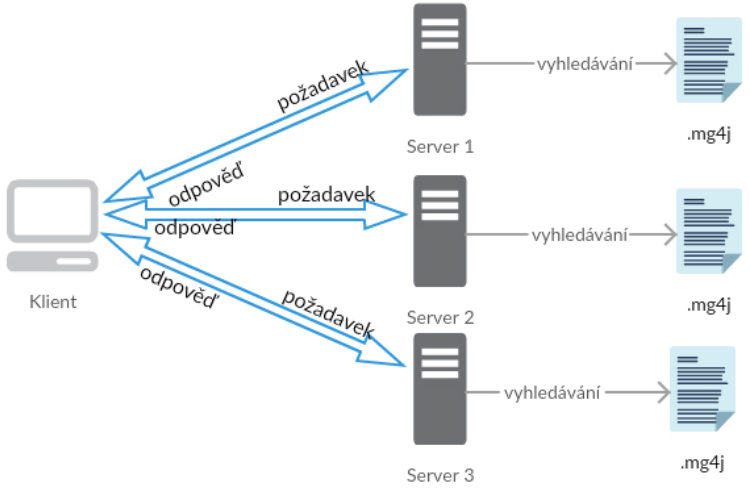
\includegraphics[scale=0.5]{obrazky-figures/ClientServerSimple.png}
    \caption{Rozdělení systému na logické části}
    \label{ClientServerSimpleLbl}
\end{figure}




\section{Návrh serverové aplikace}
\label{ServerAppProposal}
V architektuře serverové části systému není potřeba nic měnit, protože obsahuje všechny potřebné komponenty, avšak je potřeba provést značné změny ve vnitřní struktuře komponenty, která je zodpovědná za vyhledávání a komunikaci s klientskými aplikacemi. Kvůli přidaným konfiguracím\,(viz dále), je také potřeba provést změny v komponentě zodpovědné za zpracování a uchování konfigurací.

\subsection{Modifikace serverové komponenty}
Při návrhu funkcionality serverové komponenty vycházíme z požadavků definovaných v~podkapitole \ref{taskDescriptin}. Postupně si probereme klíčové body, které musejí být zohledněny v logice serverové aplikace. 

Již víme, že proces dotazování probíhá s využitím modelu klient-server. Na serveru tedy musí být \uv{vstupní bod}, ve kterém začíná proces vyhledávání. Tímto bodem je získání zprávy od klienta.


\subsection*{Přijetí zprávy}
Předpokládá se, že při sestavování dotazu s entitami, klient nemusí znát vnitřní strukturu  souborů ve formátu mg4j\,(vertkální formát) ani význam polí \emph{param0} až \emph{param9}, která popisují jednotlivé entity. Klient by měl vědět jenom to, které informace může získat, a~hodnoty, které může definovat při tvorbě dotazu. Například pro entity třídy \emph{person} může získat informaci o~místě narození  nebo může pro entitu třídy \emph{event} zjistit datum konce události\,(zároveň může nastavit tyto hodnoty pro upřesnění dotazu), ale nemusí vědět o tom, že tyto informace jsou obsaženy v poli \emph{param4} a při tvorbě dotazu bude místo \emph{param4} rovnou používat sémantické \emph{birthplace} resp. \emph{enddate}. Avšak nástroj MG4J, který se používá pro vyhledávání, potřebuje získat dotaz obsahující \emph{param4}, protože nemá informaci o sémantice jednotlivých polí. Tato skutečnost vyžaduje vytvoření prvku provádějícího mapování uživatelského dotazu v jazyce MG4J-EQL \ref{mg4jeql} na vyhledávací dotaz.


\subsection*{Vykonaní požadavku}
\label{SearchForSnpts}
Po převedení uživatelského dotazu do formátu, kterému rozumí nástroj MG4J, se musí provést rozhodování o činnosti, která se má vykonat: vyhledávaní snippetů nebo celého dokumentu. V případě požadavku na získaní snippetů je potřeba znát  posun\,(offset) v rámci kolekcí, se kterým by se mělo provádět vyhledávání. Posun by měl být součásti zprávy od~klienta. Díky posunu je možně provádět dotazovaní na \uv{další dávku} snippetů. Následně je prostřednictvím nástroje MG4J potřeba získat seznam dokumentů, ve kterých se vyskytují  uživatelským dotazem definované fragmenty a metainformace o dokumentu. Zjednodušená vizualizace myšlenky s posunem a seznamem dokumentu je znázorněna na  obrázku \ref{ListOdDocumentsLblLbl}. V~případě požadavku na získaní celého dokumentu je potřeba získat celý dokument a~metainformace o něm.


\begin{figure}[ht]
\begin{center}
	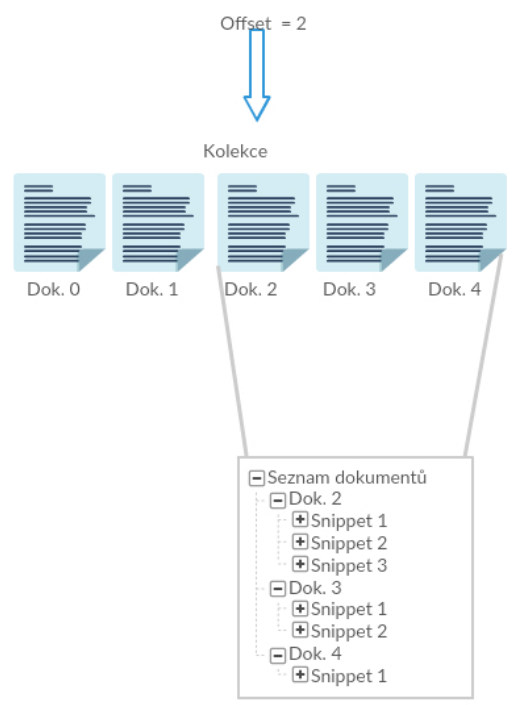
\includegraphics[scale=0.5]{obrazky-figures/OffsetInCollection.png}
\end{center}
	\caption{Posun v rámci kolekce a seznam dokumentů se snippety.}
    \label{ListOdDocumentsLblLbl}
\end{figure}


\subsection*{Zpracování vyhledaných dat}
\label{dataProcessing}
Po získaní snippetů či dokumentu na základě parametrů předaných klientem je potřeba provést zpracování. Pod pojmem \uv{zpracování} se myslí přidáni doplňkové informace požadované klientem k entitám a ne-entitám a jejich zvýraznění. Vzhledem k tomu, že podle zadání je potřeba brát zřetel na existenci webové verze klientské aplikace a vytvořit TUI verzi, je také potřeba navrhnout způsob zvýraznění entit a ne-entit tak, aby bylo možné využívat obě klientské aplikace. Při návrhu je nutné uvažovat fakt, že formát by měl být jednoduše pochopitelný uživatelem, a zároveň maximálně jednoduchý na zpracování oběma verzemi klientské aplikace. Jako formát zvýraznění lze použít prvek používaný v XML\,--\,znáčku. Značky XML jsou intuitivní pro uživatele a při volbě vhodné značky není potřeba složité zpracování na straně webové verze klientské aplikace. Při použití TUI verze klientské aplikace by uživatel neměl trávit dlouhou dobu pří vyhledávání jednotlivých entit v terminálu, a proto by tyto entity měly být, kromě zabalení do příslušné značky, také obarveny. Avšak vzhledem k tomu, že různé terminály mají různé barevné palety, je potřeba klientovi poskytovat i neobarvený text, aby se obarvení mohlo provést na straně klientské aplikace, kdy uživatel může sám konfigurovat barvy entit.


Pro webovou verzi je vhodné použití stylu\,(pojmenujeme ho HTML), ve kterém se používá značka \uv{anchor}\,(\texttt{<a>}). Použití této značky je vhodné vzhledem k možnosti definice odkazu na webovou stránku zvýrazněné entity. Všechny informace, které uživatel potřebuje, lze definovat pomocí atributů, viz výpis \ref{HTMLHightLineLbl}. U atributů ve stylu HTML\,(kromě atributů \texttt{href} a \texttt{style}) je potřeba mít předponu \uv{data-} z důvodu escapování, jelikož tag \texttt{<a>} již má předdefinovanou sémantiku pro některé atributy. 


\begin{lstlisting}[caption={Zvýraznění ve stylu HTML}, label={HTMLHightLineLbl}, captionpos=b]
<a href="http://en.wikipedia.org/wiki/John_Fisher" data-nertag="person"
data-position="17 18"...>John Fisher</a>
\end{lstlisting}
 


Při označování entit ve stylech vhodných pro TUI verzi\,(pojmenujme je ASCII a RAW) lze entity zabalit do značky dle její třídy, jak je patrné z příkladů ve výpisech \ref{RAWHightLineLbl} a \ref{ASCIIHightLineLbl}. V těchto stylech není nutné escapovat žádné atributy. Jediným rozdílem těchto dvou stylů je to, že při stylu ASCII se entita obarvuje na straně serveru a klient získává obarvenou entitu, zatímco u stylu RAW server vrátí neobarvené entity a obarvení se provádí na straně klienta.

\begin{lstlisting}[caption={Zvýraznění ve stylu RAW}, label={RAWHightLineLbl}, captionpos=b]
<person href="http://en.wikipedia.org/wiki/John_Fisher" nertag="person"
position="17 18"...>John Fisher</person>
\end{lstlisting}
 

 
 
\begin{lstlisting}[caption={Zvýraznění ve stylu ASCII}, style=base, label={ASCIIHightLineLbl}, captionpos=b]
@<person href="http://en.wikipedia.org/wiki/John_Fisher" nertag="person"@
@position="17 18"...>John Fisher</person>@
\end{lstlisting}
 


V případě, že je entita víceslovná, má každé slovo vlastní syntaktické vlastnosti. Tyto vlastnosti jsou obsaženy v hodnotě atributu a odděleny mezerou. Při označování ne-entity ve stylech RAW a ASCII se využívá značka \texttt{<field>}, ve stylu HTML se využívá \texttt{<span>}. Ne-entity se  neobarvují.



\subsection{Modifikace konfiguračního souboru a komponenty}
Změny v komponentě pro práci s konfiguracemi jsou potřebné kvůli změnám konfiguračního souboru. Jak již bylo zmíněno, serverová aplikace zvýrazňuje entity a ne-entity pomocí značek XML, které jsou různé v závislosti na požadavku klientské aplikace, což vede k přidání výchozí konfigurace stylu. Pro TUI rozhraní by se také měly použít různé barvy pro zvýraznění entit, což vynucuje přidání výchozích hodnot barev pro jednotlivé entity. Vzhledem k potřebě převedení uživatelského dotazu v jazyce MG4J-EQL do formátu, kterému rozumí nástroj MG4J, je potřeba uchovávat mapovaní mezi poli \emph{param0} až \emph{param9} a jejích sémantikou pro různý třídy entit.       


\section{Návrh klientské aplikace}
\label{ClientArchProposalLbl}
Dále je navržena klientská aplikace, která zajišťuje sbírání dat ze serverů. Přestože již existuje starší verze klientské aplikace, je nepoužitelná z důvodu značných změn serverové části a požadavků  na ní kladených. Proto byla navržena zcela nová aplikace, která je kompatibilní s novou verzí serverové části. Dále jsou probírány klíčové body, které jsou v~aplikaci zohledněny. 

\subsection*{Zpracování vstupních parametrů}
Vzhledem k vysoké míře konfigurovatelnosti je nezbytná existence souboru pro ukládání různých  konfigurací. Tato skutečnost vede k vytvoření komponenty zodpovědné za načtení, zpracování a uchovávání parametrů z příkazové řádky a konfiguračního souboru.


\subsection*{Zajištění komunikace se servery}
Po zpracování parametrů je potřeba navázat komunikaci se servery.  Obě verze klientské aplikace musí komunikovat se servery stejným způsobem, což vede k tvorbě společné komponenty pro webovou i TUI verzi. Hlavními úlohami komponenty jsou zajištění připojení a~komunikace se servery.

Vzhledem k tomu, že soubory ve formátu mg4j jsou rozdistribuovány mezi více servery, jejichž množství není předem známo, je postupné dotazování se nevyhovující z důvodu časové neefektivnosti. Pro zajištění maximální rychlosti je nutné použití více vláken s tím, že každé vlákno komunikuje s jedním serverem. Každé vlákno vytváří zprávu pro svůj server a v~případě, že odpověď neodpovídá očekávané\,(nebyl vrácen dostatečný počet výsledků), provede klientská aplikace  opakované dotazování s případně modifikovanou zprávou. Také je nezbytné zajistit synchronizovaný zápis odpovědí do seznamu. Aplikace by měla zajistit i implicitní vypočítání hodnoty posunu v~rámci kolekce pro každý server v případě získání \uv{další dávky} snippetů.

\subsection*{Zpracování a výpis odpovědi}
Po získání odpovědí od serverů je před jejich výpisem zapotřebí provést jejich případné zpracování. To vede k tvorbě patřičné komponenty. Servery vrátí velké množství informací:~vlastní obohacená data, svoji adresu, posun v rámci kolekcí, různé meta-informace o~dokumentech, ve kterých byla tato data nalezena\,(titulek, odkaz apod.) a další. Úlohou této komponenty je pravě formátování těchto informací na základě nastavení uživatele, před samotným výpisem.


Po zpracování je potřeba vytisknout naformátované odpovědi. Tento úkol přebírá další komponenta, která je zodpovědná za tisk. Vzhledem k existenci dvou verzí klientské aplikace\,(tedy dvou různých přístupů k tisku zpracovaných odpovědí) je v komponentě pro tisk vhodné použití návrhového vzoru \uv{Vkládání závislostí}\,(angl. Dependency injection). 


Jak již bylo nastíněno v návrhu serverové aplikace, může nastat případ, kdy se klientská aplikace spouští z terminálů, který nemá dostatečně rozsáhlou barevnou paletu pro obarvení entit výchozími barvami na straně serveru. V těchto případech uživatel může požádat server o vrácení neobarvených entit, aby provedl obarvení sám podle schopnosti terminálu, ve~kterém pracuje. Aby uživatel mohl sám definovat barvy pro jednotlivé entity, je potřeba mít plnou paletu barev na straně klienta, ze které může uživatel používat barvy podporované svým terminálem. Možnost definovat barvy vede k vytváření komponenty, která mapuje barvy v přirozeném jazyce na číselné hodnoty, do kterých jsou barvy zakódované\,(černé barvě odpovídá \uv{\texttt{$\backslash$u001B[30m}} apod.). 



\subsection*{Uchování informace pro dotaz na \uv{další dávku} dat}
Aby byla aplikace schopna provádět dotazování na \uv{další dávku} dat, je potřeba uchovávat posun v rámci kolekce jednotlivých serverů. Na základě počtu vrácených snippetů lze rozhodnout, jestli server ještě má v kolekcích další snippety. V případě, že server vrátí minimálně očekávané množství snippetů, lze dojít k závěru, že je potenciálně možné vrátit další dávku, jinak nemá dostatečné množství snippetů v kolekcích a nemá cenu se  znovu dotazovat. 

Pro zajištění schopnosti získat další dávky snippetů je potřeba  po ukončení komunikace provést kontrolu počtů vrácených snippetů z jednotlivých serverů a vynechat ty, které vrátily méně snippetů, než po nich bylo požadováno. Adresy těchto serverů se zapisují do~mapy jako páry \uv{klíč-hodnota}, kde klíč je roven adrese serveru a hodnotou tohoto klíče je posun v rámci kolekcí na daném serveru. Před ukončením je potřeba provést serializaci této mapy. 

V případě požadavku na získání \uv{další dávky} dat se provádí deserializace této mapy a~další dotazování se provádí jenom na servery, které jsou uložené jako klíče v této mapě.




\chapter{Implementace serverové a klientské části}
\label{chapter6}

Tato kapitola se věnuje detailnímu popisu implementace serverové a klientské části. Následující text pojednává o  změnách v jednotlivých komponentách systému na základě výše uvedeného návrhu.   


\section{Implementace serverové aplikace}
\label{serverSideImplem}
Při implementaci vycházíme z návrhu uvedeného v podkapitole \ref{ServerAppProposal}. Jednotlivé balíky jsou popsány postupně od začátku běhu serverové aplikace. 

\subsection*{Příprava serveru}

Běh aplikace začíná v balíku \textbf{cli}, třídě \emph{Cli}. Nejprve se provádí zpracování vstupních parametrů z příkazové řádky, načtení a ukládání konfigurací z konfiguračního souboru. Za~zpracování a ukládaní konfigurace je zodpovědná třída \emph{ConfigAndPerformate} z balíku  \textbf{config}. Po~zpracování se vytváří hluboká kopie\,(deep copy) instance této třídy, která se mění v~závislosti na požadavcích klienta\,(když jsou odlišné od výchozích). Uchování jedné kopie s~původními hodnotami zajišťuje možnost použití výchozích konfigurací. Pro zjednodušení přístupu ke~konfiguracím se instance \emph{ConfigAndPerformate} ukládají do statických proměnných abstraktní třídy \emph{ConfigHolder} z balíku \textbf{config}. Díky tomu je možné použití obou instancí z~libovolného místa v programu. Dále se na základě parametrů zadaných při spouštění provede rozhodování o úloze, která se má provést. V případě této práce se spouští úloha označená jako \emph{serve}. Další běh programu pokračuje v balíku \textbf{queryserver}, ve třídě \emph{CommandServe}.

Ve třídě \emph{CommandServe} se provádí načtení kolekcí, načtení jednotlivých polí\,(\emph{position}, \emph{lemma}, \emph{token} apod.) z konfiguračního souboru a začíná očekávání zpráv od klientských aplikací.

\subsection*{Příjem zprávy}
Server obdrží zprávu od klienta ve formátu JSON a provede přeformátování pole \emph{query}\,(dotaz definující fragment v jazyce MG4J-EQL). Za přeformátování je zodpovědná třída \emph{QueryTranslater} ze stejného balíku. V závislosti na třídě entity\,(\emph{person}, \emph{event} nebo jiné) se provádí mapování sémantických hodnot \emph{birthdate}, \emph{name}, \emph{profession} a dalších na jednotlivá pole \emph{param0} až \emph{param9}. Po mapování se uživatelský dotaz přepíše do formátu srozumitelného nástroji MG4J. Po překladu se provádí rozhodování o úloze: vrácení celého dokumentu nebo požadovaného množství snippetů. 

\subsection*{Vyhledávání snippetů}
\label{SearchSnippetsLbl}
V případě dotazu na určité množství snippetů se~provádí odhad počtu dokumentů, ve kterých se~nachází požadovaná množina snippetů. Prvotní odhadovaní množství dokumentů se~musí provést kvůli tomu, že nástroj MG4J neumí vyhledat samotné snippety, ale pouze dokumenty a množiny snippetů v rámci těchto dokumentů\,(obr. \ref{ListOdDocumentsLblLbl}). Po provedení vyhledání v~kolekci s počátečním posunem\,(viz podkapitola \ref{ServerAppProposal}) určeným klientskou aplikací se~provádí zpracování snippetů z dokumentů. Po zpracování se provádí kontrola počtu zpracovaných snippetů. V případě, že je počet menší než množství požadované uživatelem a~existují další dokumenty, které mohou obsahovat snippety, se provádí opakované hledání, nyní však s~dalším posunem. Po získání požadované množiny snippetů nebo v případě absence dalších snippetů, se již zpracované snippety  vracejí klientské aplikaci jako odpověď. Logika této části je znázorněná na diagramu aktivit na obrázku \ref{ActivityDiagramSnptsProcess}. 




\begin{figure}[H]
\hspace{-0.8cm}
	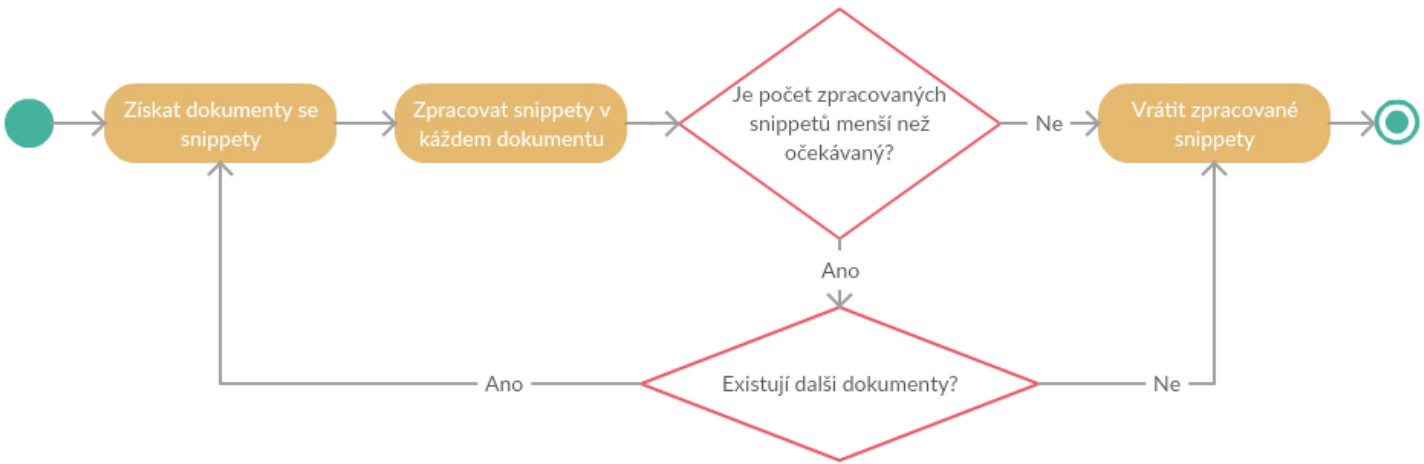
\includegraphics[scale=0.33]{obrazky-figures/SnippetsProcessActivity.png}
	\caption{Diagram aktivit sbírání snippetů}
    \label{ActivityDiagramSnptsProcess}
\end{figure}


\subsection*{Příprava snippetů}

Vlastní uchování a zpracování snippetů se provádí ve třídě \emph{SnippetHolder}. Při instanciaci třída \emph{SnippetHolder} očekává dokument s množinou snippetů. Dokument představuje objekt, který obsahuje titulek, odkaz na webovou stránku, ze které byl stažen, množinu snippetů a~pro každý token ve snippetu hodnoty jednotlivých polí relevantních pro daný token. Třída \emph{SnippetHolder} uchovává dokument ve struktuře  \emph{\uv{snippets-parts-fields}}. V této struktuře je \emph{\uv{snippets}}  seznamem snippetů, ve kterém se každý snippet skládá z částí\,(\emph{\uv{parts}}), kde každá část představuje jednu logickou jednotku\,(entita nebo ne-entita), která se skládá ze~seznamu polí\,(\emph{\uv{fields}}). Každé pole\,(\emph{field}) reprezentuje mapu hodnot jednotlivých syntaktických a~sémantických informací, které patří jednomu tokenu. Vzhledem k tomu, že~se~některé entity skládají z více slov, provádí se sloučení polí, které patří jedné entitě, do jedné části. Pro lepší pochopení slouží obrázek v příloze \ref{SnippetsPartsFieldsLbl}. 



\subsection*{Zpracování snippetů}
\label{SnippetsProcessingLbl}
Po uložení snippetů do struktury \emph{\uv{snippets-parts-fields}} začíná zpracování. Nejprve se extrahuje hodnota pole definovaného uživatelem\,(z čeho se vytváří výsledný text) a další zpracování se následně provádí ve třídě \emph{ConfigAndPerformate}. Při zpracování se každá část každého snippetu zpracovává interpretem jazyka \emph{Lisp}, který filtruje syntaktické a sémantické  informace, které nebyly požadované klientem. Po filtrování se provádí rozhodování o~způsobu zvýraznění\,(stylu). Z~podkapitoly \ref{dataProcessing} víme, že server nabízí možnost volby jednoho ze třech stylů HTML, ASCII a RAW.  V případě stylu ASCII provádí obarvení na~straně serveru. Názvy barev jsou uloženy v konfiguračním souboru. Pro mapování názvů barev na jejích číselné hodnoty slouží výčtový typ \emph{Color} z balíku \textbf{queryserver}.  Po obarvení se jednotlivé části skládají do plynulého textu.

Pro lepší pochopení struktury serverové části slouží diagram balíků na obrázku \ref{ServerApplicationLbl}. Podrobnější diagram tříd je uveden v příloze \ref{ClassDiagramServerLbl}. 

\begin{figure}[ht]
	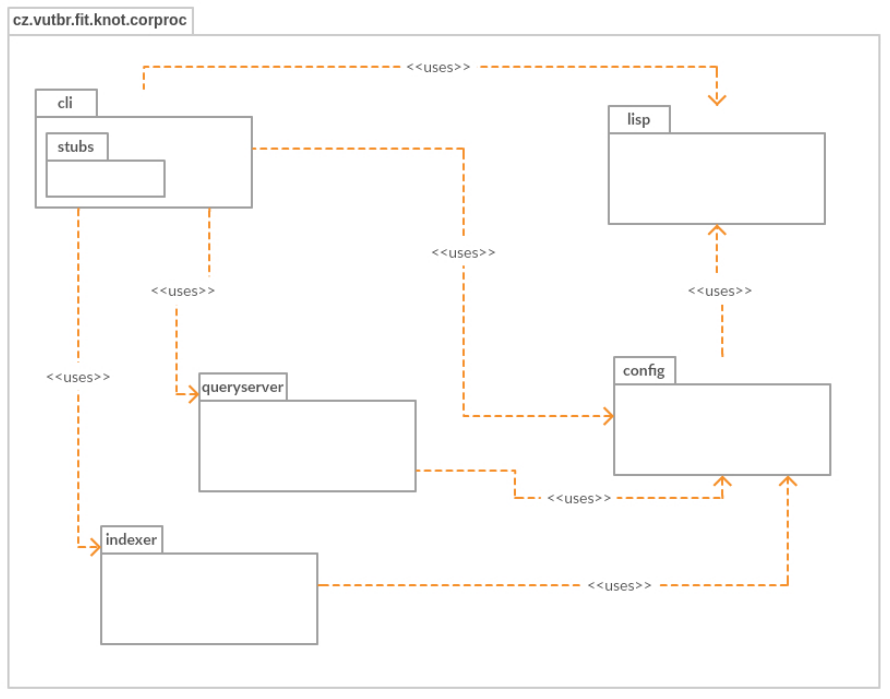
\includegraphics[scale=0.5]{obrazky-figures/ServerPackageDiagram.png}
    \caption{Diagram balíků serverové aplikace}
    \label{ServerApplicationLbl}
\end{figure}




\subsection{Vyhledávání a zpracování dokumentu}
V případě požadavku na získání konkrétního  dokumentu by uživatel měl definovat identifikátor dokumentu v kolekci a identifikátor kolekce, ve které se dokument nachází. Identifikátor dokumentu a identifikátor kolekce jsou částmi zprávy, kterou vrací server pří dotazu na~množinu snippetů. Předpokládá se, že dřív, než uživatel zažádá o celý dokument, požádá server o vrácení množiny snippetů.

Nástroj MG4J vrací celý dokument a meta-informace o něm. Dále se provede stejný postup jako v případě dotazu na množinu snippetů: dokument se uchová do třídy \emph{SnippetHolder}, provede se přidáni různých informací entitám a ne-entitám, které se následně balí do patřičné značky a obarví patřičnými barvami a zpracovaný dokument se vrací klientovi.  

\section{Implementace klientské aplikace}
Při implementaci vycházíme z návrhu uvedeného v podkapitole \ref{ClientArchProposalLbl}. Popis implementace opět odpovídá běhu programu.

\subsection*{Příprava ke komunikaci}
Běh programu začíná v balíku \textbf{main}, ve třídě \emph{Main}. V této třídě se provádějí přípravné kroky pro následnou komunikaci. Nejprve se provádí zpracování vstupních parametrů, načtení a~zpracování konfigurací z konfiguračního souboru. Za zpracování těchto vstupních informací je zodpovědná třída \emph{Parameters} z balíku \textbf{parameters}. Pro pohodlnou práci se~tyto informace uchovávají do mapy. Třída \emph{Parameters} je adaptérem pro práci s touto mapou a~poskytuje metody pro získání a nastavení hodnot na základě klíče. Také se provádí deserializace mapy se servery a posuny v případě požadavku na získání \uv{další dávky} dat.

Po načtení a zpracování parametrů a konfigurací se provádí instanciace třídy \emph{ResponseProcessor} z balíku \textbf{processor}. Tato třída je zodpovědná za zpracování odpovědí získaných od serverů. Po instanciaci třídy \emph{ResponseProcessor} se provádí instanciace třídy \emph{ResponsePrinter} z balíku  \textbf{printer}, která vypisuje zpracované odpovědi. Poté se instance třídy \emph{ResponseProcessor} vkládá do instance třídy \emph{ResponsePrinter}.

Dalším krokem pří přípravě ke komunikaci je instanciace a nastavení třídy \emph{QueryParameters} z balíku \textbf{query}. Třída obsahuje množinu parametrů, které jsou nezbytné pro komunikaci se servery. Je také adaptérem zastřešujícím mapu, ve které se uchovávají parametry. Posledním krokem před začátkem komunikace je instanciace třídy \emph{QueryModule} z~balíku \textbf{query}.


\subsection*{Začátek komunikace, balík \uv{query}}
Balík \textbf{query} je jádrem celé klientské aplikace. Díky způsobu implementace je použitelný pro obě verze klientské aplikace. Balík se skládá ze čtyř tříd: \emph{Query}, \emph{QueryModule}, \emph{QueryParameters} a \emph{QueryThread}. Komunikace začíná ve třídě \emph{QueryModule}. Pro validní komunikaci získává třída přístup k:
\begin{enumerate}
\item instanci třídy \emph{QueryParameters}, obsahující parametry potřebné pro komunikaci,

\item seznamu serverů, se kterými se navazuje komunikace\,(seznam serverů se nachází v~souboru, který je definován parametrem při spouštění programu),

\item seznamu objektů typu JSON, do kterého se nahrávají odpovědi od serverů,

\item deserializované mapě se servery a posuny v rámci jednotlivých serverů,

\item instanci třídy \emph{ResponsePrinter} zodpovědné za výpis zpracovaných odpovědí.
\end{enumerate}

V případě, že deserializovaná mapa není \emph{null}, seznam serverů z druhého bodu nahrazuje klíče této mapy\,(tím se zajistí komunikace jenom se servery, které potenciálně mohou vrátit snippety). Dále se provádí cyklus přes všechny adresy serverů. Při každé iteraci se~vytváří instance třídy  \emph{QueryThread}, která vytváří zprávy pro server. Veškerá příprava ke~komunikaci a vlastní komunikace se serverem se koná v samostatném vlákně. Instance třídy \emph{QueryThread} získává přístup k:
\begin{enumerate}
\item seznamu, do kterého se nahrávají odpovědi,

\item instanci třídy \emph{QueryParameters},

\item adrese pro navázání komunikace se serverem,

\item posunu v rámci kolekce serveru,

\item číslo definující počet očekávaných snippetů od konkrétního serveru.
\end{enumerate}

Instance \emph{QueryThread} vytváří zprávu obsahující všechny potřebné informace, jako například dotaz v jazyce MG4J-EQL, styl\,(ASCII, HTML nebo RAW), počet snippetů očekávaných od serveru apod. V případě požadavku na získání celého dokumentu vytváří zprávu obsahující identifikátor dokumentu a kolekci, ve které se dokument nachází. Po vytvoření zprávy se provádí instanciace třídy \emph{Query}.

Instance třídy \emph{Query} získává zprávu vytvořenou třídou \emph{QueryThread} a adresu serveru, kterému  odesílá vytvořenou zprávu. Po odeslání zprávy čeká na odpověď po dobu přednastavenou při spuštění programu. Po obdržení odpovědi tuto odpověď doplní o počet očekávaných a reálně získaných snippetů\,(jsou zapotřebí k tomu, aby se daly určit servery, které potenciálně mohou vrátit další snippety). Také počítá absolutní posun v rámci kolekce\,(sečte počáteční posun a posun získaný od serveru v odpovědi).  Modifikovanou odpověď vrací instanci \emph{QueryThread}, ve které byla vytvořena. \emph{QueryThread} zapisuje odpověď do seznamu s odpověďmi, který je sdílený mezi všemi vlákny. V případě, že se komunikace se serverem jíž konala, dopisuje nově získané snippety do objektu, který obsahoval snippety z dřívějších komunikací se serverem, a obnovuje hodnotu počátečního posunu v rámci kolekce.

Jakmile všechna vlákna skončí komunikaci se servery, běh programu pokračuje v hlavním vlákně, ve třídě \emph{QueryModule}. Hlavní vlákno iniciuje zpracování a výpis odpovědí zavoláním metody třídy   \emph{ResponsePrinter}. V případě že celkový počet vrácených snippetů ze všech serverů neodpovídá očekávanému počtu, opakovaně se provede sesbírání snippetů ze severů, které potenciálně mohou obsahovat jejich další dávku. 

\subsection*{Zpracování a výpis dat}
Jak jíž bylo zmíněno, za zpracování dat je odpovědná třída \emph{ResponsePrinter}. Třída používá instanci \emph{ResponseProcessor} pro zpracování snippetů či celého dokumentu. Třída přijímá seznam objektů ve formátu JSON a postupně je ve smyčce zpracovává a vypisuje na~standardní výstup. Během zpracování se provádí obarvení entit barvami definovanými uživatelem v konfiguračním souboru\,(v případě stylu RAW mapování názvů barev na číselné hodnoty provádí výčtový typ \emph{Color} z balíku \textbf{colorizer}) a sestavování hlavičky\,(číslo dokumentu, titulek, odkaz apod.). Zpracovaný text se vypisuje na standardní výstup. Po~zpracování snippetů se veškeré snippety mažou z objektu odpovědi, avšak vlastní objekt se nemaže pro případ opakované komunikace se serverem\,(pří opakované komunikaci se nové snippety znovu zapisují do již uloženého objektu). Mazaní zpracovaných snippetů je nezbytné kvůli riziku překročení limitu paměti.

V případě požadavku na celý dokument se celá posloupnost kroků opakuje. Rozdíl je v tom, že požadavek na získání celého dokumentu se posílá jenom jednomu serveru, který tento dokument obsahuje. Adresu serveru, identifikátor dokumentu a identifikátor kolekce definuje uživatel pomocí parametrů příkazové řádky. Pro lepší představu o vnitřní struktuře viz obrázek \ref{ClientPackageDiargamLbl}. V příloze \ref{ClientClassDiagrameLbl} je také podrobnější diagram tříd.



\begin{figure}[H]
\begin{center}
	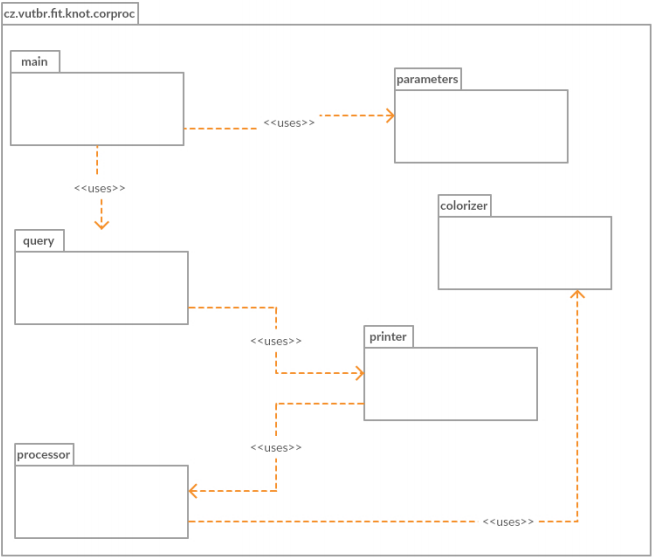
\includegraphics[scale=0.5]{obrazky-figures/ClientPackageDiagram.png}
\end{center}
	\caption{Diagram balíků klientské aplikace}
    \label{ClientPackageDiargamLbl}
\end{figure}



\chapter{Testování a experimentování}
\label{chapter7}

Tato kapitola se věnuje popisu testování vyvinutých částí. Testování je rozděleno na dvě fáze. V první fázi se provádí ověřování správnosti softwaru, ve druhé se provádí sbíraní statistik, díky kterým lze odvodit některé závislosti a vztahy.       


 

\section{Plán testování}
\label{testPlan}
V první fázi zjišťujeme:
\begin{enumerate}
\item jestli systém opravdu rozlišuje mezi požadavkem na získaní snippetů a požadavkem na získaní dokumentu,

\item jestli systém při dotazu na získaní snippetů opravdu vrací množství požadovaných snippetů a při dotazu na získaní dokumentu požadovaný dokument,

\item jestli systém opravdu umí rozlišit styly ASCII, HTML a RAW,

\item jestli systém opravdu provádí správné mapování sémantických atributů jednotlivých entit na poli v souborech ve formátu mg4j,

\item jestli systém správně doplní syntaktické a sémantické informace podle požadavku.
\end{enumerate}
V druhé fázi ověřujeme následující závislosti:

\begin{enumerate}
\item závislost doby vyhledávání na množství dat, ve kterých se provádí vyhledávání,

\item závislost doby vyhledávání na množství snippetů požadovaných při vyhledávání,

\item závislost doby vyhledání na složitosti dotazu,

\item závislost mezi množstvím snippetů a množstvím fragmentů, resp. kolik fragmentů se vyskytuje v jednom snippetu,

\item závislost mezi množstvím  fragmentů\,(snippetů) a množstvím dokumentů, které obsahují tyto fragmenty\,(snippety), resp. kolik fragmentů\,(snippetů) se vyskytuje v jednom dokumentu.
\end{enumerate}
Aby bylo možné určit tyto závislosti, bylo provedeno měření následujících údajů:
\begin{enumerate}
\item doba vyhledávání požadovaného množství snippetů,
\item množství vrácených snippetů,
\item množství výskytů fragmentů odpovídajících dotazu,
\item množství dokumentů, ve kterých se provedlo vyhledání požadovaného množství snippetů.
\end{enumerate}

\section{Popis testovacích dat}

Pro testovaní byly zvoleny tři různě velké disjunktní množiny souborů ve formátu mg4j. Množina \emph{collPart001} o celkové velikosti 2\,271\,582KB\,(2.27GB)  se skládá ze čtyřech souborů, které dohromady obsahují 38\,681 dokumentů. Množina \emph{collPart002} o velikostí 4\,545\,191KB (4.55GB) se skládá z osmi souborů a celkově 78\,032 dokumentů. Množina \emph{collPart003} se~skládá z~deseti souborů o celkové velikosti 5\,673\,297KB\,(5.67GB) a obsahuje 98\,275 dokumentů. Indexy vytvořené pro vyhledávaní v kolekcích jsou stejně velké, cca. 24KB. Testování bylo provedeno na školním výzkumném serveru \emph{athena1}\,(2$\times$Intel Xeon 6/12 jader, 15MB cache E5-2630vz, 128GB RAM, 8$\times$6TB disk v SW RAID6).

\section{Průběh testování}
Testování se provedlo na třech různých dotazech: 
\begin{enumerate}
\item \emph{influenced}

\item \emph{nertag:date}

\item \emph{nertag:date < nertag:person}
\end{enumerate} 
Pro každý dotaz se provedlo několik pokusů s postupným zvětšením množiny očekávaných snippetů. Během testování byly naměřeny údaje uvedené v podkapitole \ref{testPlan}, po provedení dotazování byly výsledky seřazeny do tabulek \ref{influencedStats}, \ref{nertagdateStats} a \ref{nertagdatenertagpersonStats}. Při dotazování se střídaly konfigurace stylů a obarvení jednotlivých entit. Měnily se také požadavky na získání různých syntaktických a sémantických informací. Pro ověření čtvrtého bodu první fáze byly zvlášť provedeny dotazy uvedené v podkapitole \ref{mg4jeql}. Také bylo provedeno deset dotazování na získání různých dokumentů, pro ověření prvního a druhého bodu první fáze. Výsledky každého dotazu byly přesměrovány do souboru a následně analyzovány. 


Sloupec \textbf{Snippety} obsahuje množství získaných snippetů, sloupec \textbf{Fragmenty} obsahuje množství fragmentů, které odpovídají dotazu, a  sloupec \textbf{Dokumenty} ukazuje počet dokumentů, ve kterých byly snippety nalezeny.  

\begin{table}[!ht]
\begin{tabular}{|c|c|c|c|c|c|}
\hline
\textbf{Kolekce} & \textbf{Doba\,(sec.)} & \textbf{Oček. snippety} & \textbf{Snippety} & \textbf{Fragmenty} & \textbf{Dokumenty} \\
\hline
\emph{collPart001} & 3.950 & 100 & 105 & 106 & 89 \\
\hline
\emph{collPart001} & 4.347 & 150 & 150 & 152 & 129 \\
\hline
\emph{collPart001} & 5.309 & 200 & 212 & 214 & 179 \\
\hline
\emph{collPart001} & 6.297 & 250 & 252 & 254 & 209 \\
\hline
\emph{collPart001} & 7.165 & 300 & 306 & 308 & 248 \\
\hline
\emph{collPart001} & 8.126 & 500 & 332 & 334 & 264 \\
\hline
\emph{collPart001} & 7.658 & 1500 & 332 & 334 & 264 \\
\hline
\emph{collPart001} & 7.980 & all & 332 & 334 & 264 \\
\hline\hline
%%%%%%%%%%%%%%%%%%%%%%%%%%%%%%%%%%%%%%%%%%%%%%%
\emph{collPart002} & 3.411 & 100 & 107 & 109 & 80 \\
\hline
\emph{collPart002} & 4.455 & 150 & 164 & 161 & 120 \\
\hline
\emph{collPart002} & 5.143 & 200 & 205 & 210 & 160 \\
\hline
\emph{collPart002} & 5.830 & 250 & 254 & 259 & 200 \\
\hline
\emph{collPart002} & 7.042 & 300 & 308 & 313 & 250 \\
\hline
\emph{collPart002} & 12.263 & 500 & 507 & 515 & 408 \\
\hline
\emph{collPart002} & 17.172 & 1500 & 656 & 667 & 524 \\
\hline
\emph{collPart002} & 17.111 & all & 656 & 667 & 524 \\
\hline\hline
%%%%%%%%%%%%%%%%%%%%%%%%%%%%%%%%%%%%%%%%%%%%%%%%%%%%%
\emph{collPart003} & 3.117 & 100 & 106 & 111 & 90\\
\hline
\emph{collPart003} & 4.468 & 150 & 157 & 160 & 130\\
\hline
\emph{collPart003} & 5.832 & 200 & 208 & 212 & 170\\
\hline
\emph{collPart003} & 6.940 & 250 & 258 & 262 & 210\\
\hline
\emph{collPart003} & 7.336 & 300 & 304 & 308 & 249\\
\hline
\emph{collPart003} & 11.227 & 500 & 501 & 513 & 418 \\
\hline
\emph{collPart003} & 16.171 & 1500 & 856 & 881 & 712 \\
\hline
\emph{collPart003} & 21.763 & all & 856 & 881 & 712 \\
\hline
\end{tabular}
\caption{Statistiky při dotazu \emph{influenced}}
\label{influencedStats}
\end{table}


\clearpage

\begin{table}[!ht]
\begin{tabular}{|c|c|c|c|c|c|}
\hline
\textbf{Kolekce} & \textbf{Doba\,(sec.)} & \textbf{Oček. snippety} & \textbf{Snippety} & \textbf{Sragmenty} & \textbf{Dokumenty} \\
\hline
\emph{collPart001} & 1.110 & 100 & 168 & 201 & 20 \\
\hline
\emph{collPart001} & 2.704 & 500 & 506 & 599 & 135\\
\hline
\emph{collPart001} & 7.085 & 1500 & 2048 & 2048 & 472 \\
\hline
\emph{collPart001} & 10.611 & 5000 & 5257 & 6423 & 1212 \\
\hline
\emph{collPart001} & 22.639 & 10000 & 14712 & 12264 & 2770 \\
\hline
\emph{collPart001} &  97.409 & 50000 & 62850 & 51608 & 11930 \\
\hline
\emph{collPart001} &  223.234 & all & 66054 & 80354 & 15010 \\
\hline\hline
%%%%%%%%%%%%%%%%%%%%%%%%%%%%%%%%%%%%%%%%%%%%%%%%%%%
\emph{collPart002} & 1.375 & 100 & 112 & 142 & 38 \\
\hline
\emph{collPart002} & 3.399 & 500 & 525 & 757 & 143 \\
\hline
\emph{collPart002} & 7.305 & 1500 & 1572 & 2157 & 382 \\
\hline
\emph{collPart002} & 11.080 & 5000 & 5264 & 6787 & 1212 \\
\hline
\emph{collPart002} & 21.409 & 10000 & 11960 & 14810 & 2779 \\
\hline
\emph{collPart002} & 97.962 & 50000 & 51681 & 63400 & 11951 \\
\hline
\emph{collPart002} & 359.595 & all & 130786 & 160612 & 30078\\
\hline\hline
%%%%%%%%%%%%%%%%%%%%%%%%%%%%%%%%%%%%%%%%%%%%%%%%%%%%
\emph{collPart003} & 1.373 & 100 & 133 & 166 & 45 \\
\hline
\emph{collPart003} & 2.241 & 500 & 503 & 600 & 150 \\
\hline
\emph{collPart003} & 8.080 & 1500 & 2466 & 3290 & 462 \\
\hline
\emph{collPart003} & 17.201 & 5000 & 5226 & 6760 & 1184 \\
\hline
\emph{collPart003} & 31.037 & 10000 & 11380 & 14059 & 2730\\
\hline
\emph{collPart003} & 60.582 & 50000 & 52677 & 67095 & 11958\\
\hline
\emph{collPart003} & 397.242 & all & 161494 & 201415 & 37946\\
\hline
\end{tabular}

\caption{Statistiky při dotazu \emph{nertag:date}}
\label{nertagdateStats}
\end{table}

\clearpage

\begin{table}[!ht]
\begin{tabular}{|c|c|c|c|c|c|}
\hline
\textbf{Kolekce} & \textbf{Doba\,(sec.)} & \textbf{Oček. snippety} & \textbf{Snippety} & \textbf{Fragmenty} & \textbf{Dokumenty} \\
\hline
\emph{collPart001} & 1.944 & 100 & 110 & 110 & 20 \\
\hline
\emph{collPart001} & 5.409 & 500 & 502 & 502 & 193\\
\hline
\emph{collPart001} & 14.820 & 1500 & 1777 & 1777 & 568 \\
\hline
\emph{collPart001} & 25.099 & 5000 & 5155 & 5155 & 1991 \\
\hline
\emph{collPart001} & 53.769 & 10000 & 10912 & 10912 & 3798 \\
\hline
\emph{collPart001} &  125.272 & 50000 & 24840 & 24840 & 8904 \\
\hline
\emph{collPart001} &  217.301 & all & 24840 & 24840 & 8904 \\
\hline\hline
%%%%%%%%%%%%%%%%%%%%%%%%%%%%%%%%%%%%%%%%%%%%%%%%%%%%%%%5
\emph{collPart002} & 1.959 & 100 & 135 & 135 & 38 \\
\hline
\emph{collPart002} & 4.937 & 500 & 517 & 517 & 163 \\
\hline
\emph{collPart002} & 12.688 & 1500 & 1722 & 1722 & 568 \\
\hline
\emph{collPart002} & 26.670 & 5000 & 5264 & 6787 & 1891 \\
\hline
\emph{collPart002} & 52.096 & 10000 & 10302 & 10302 & 3769 \\
\hline
\emph{collPart002} & 242.854 & 50000 & 46789 & 46789 & 17662 \\
\hline
\emph{collPart002} & 359.595 & all & 46789 & 46789 & 17662\\
\hline\hline
%%%%%%%%%%%%%%%%%%%%%%%%%%%%%%%%%%%%%%%%%%%%%%%%%%%%%%%%%
\emph{collPart003} & 2.057 & 100 & 129 & 129 & 52 \\
\hline
\emph{collPart003} & 5.672 & 500 & 520 & 520 & 192 \\
\hline
\emph{collPart003} & 17.307 & 1500 & 1511 & 1511 & 461 \\
\hline
\emph{collPart003} & 29.827 & 5000 & 5161 & 5161 & 1979 \\
\hline
\emph{collPart003} & 57.079 & 10000 & 10288 & 10288 & 3788\\
\hline
\emph{collPart003} & 265.279 & 50000 & 51107 & 51107 & 18878\\
\hline
\emph{collPart003} & 529.347 & all & 60249 & 60249 & 22553\\
\hline
\end{tabular}

\caption{Statistiky při dotazu \emph{nertag:date < nertag:person}}
\label{nertagdatenertagpersonStats}
\end{table}





\section{Vyhodnocení výsledků}

Výsledky získané v průběhu testování byly zpracovány tak, že nejprve byla provedena analýza výsledků získaných v první fázi testování, a následné byly odvozeny závislosti z druhé fáze.

\subsection{První fáze testování}
Prvním bodem, který bylo zapotřebí ověřit v první fázi, bylo ověření, zda systém opravdu umí rozlišit mezi požadavkem na množinu snippetů a požadavkem na dokument. Během testování se střídaly požadavky na získání množiny snippetů a dokumentu a systém vždy vracel buď snippety nebo dokument. Lze tedy tvrdit, že systém správně rozlišuje požadavky a vrací patřičné výsledky.

Dalším bodem bylo ověření množství očekávaných snippetů a ověření správně vráceného dokumentu.  Z výsledků v tabulkách \ref{influencedStats}, \ref{nertagdateStats} a  \ref{nertagdatenertagpersonStats}  je jasné, že v případě dostatečného množství snippetů v kolekcích systém vrací minimálně požadované množství snippetů. Systém vrací méně snippetů pouze v případě absence požadovaného množství snippetů v kolekcích. Pro ověření správnosti vráceného dokumentu stačilo provést vyhledání patřičného snippetu ve vráceném dokumentu. Během testování systém vždy vracel dokument, který opravdu obsahoval hledaný snippet.

Třetím bodem bylo ověření schopnosti systému vrátit snippety či dokument ve správném stylu. Během testování se střídaly styly HTML, ASCII a RAW. Při každé změně stylu systém obaloval entity\,(ne-entity) do očekávaných značek a prováděl obarvení patřičnými barvami.

Čtvrtým bodem bylo ověření schopnosti systému správně namapovat sémantické atributy entit na jednotlivá pole v souborech ve formátu mg4j. Jako výsledek systém vždy vracel snippety obsahující zmínku o Johnovi Fisherovi a snippety obsahující děje se začátkem v~roce 1940 a koncem 1949.

V pátém kroku byla ověřena schopnost systému správně doplnit entity a ne-entity o~syntaktické a sémantické informace. Během testování byly o entitě třídy \emph{person} získány některé syntaktické informace\,(pozice ve větě a slovní druh) a  všechny sémantické informace\,(jméno, pohlaví, datum narození apod.). Systém vždy vracel očekávané hodnoty.  


\subsection{Druhá fáze testování}
Prvním bodem v druhé fázi bylo určení závislosti doby vyhledání na množství dat, ve~kterých se vyhledávání provádí. Pro určení závislosti bylo potřeba sestavit tabulku průměrné doby vyhledávání stejného dotazu v různých kolekcích \ref{avgTime} a na základě této tabulky sestrojit graf \ref{size_time}.

\begin{table}[H]
\centering
\begin{tabular}{|c|c|c|c|}
\hline
\textbf{Dotaz} & \textbf{collPart001} & \textbf{collPart002} & \textbf{collPart003}\\
\hline
\emph{influenced} & 6.122s &  7.902s & 7.870s \\
\hline
\emph{nertag:date} & 23.593s & 23.755s & 20.086s\\
\hline
\emph{nertag:date < nertag:person} & 37.719s & 56.867s & 62.870s \\
\hline
\end{tabular}
\caption{Průměrné doby vyhledání pro jednotlivé dotazy}
\label{avgTime}
\end{table}

\begin{figure}[H]
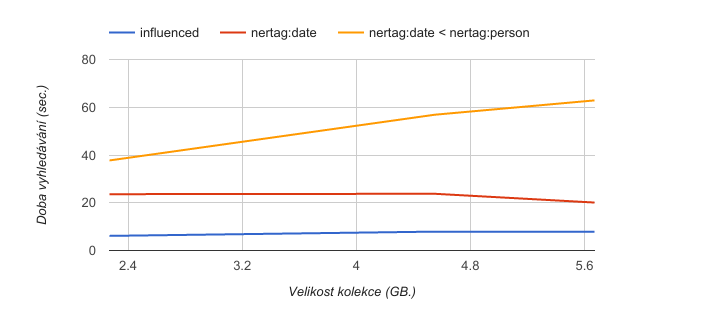
\includegraphics[scale=0.7]{obrazky-figures/size_time.png}
\caption{Grafy závislosti mezi velikosti kolekce, ve které se vyhledává a dobou vyhledávání}
\label{size_time}
\end{figure}

Na základě grafu lze usoudit, že doba nezávisí na velikosti dat, ve kterých se provádí vyhledávání.  

Druhým bodem je zjistit závislost doby vyhledávání na množství snippetů požadovaných k vyhledání. Pro odvození závislosti byly sestaveny  grafy pro každý dotaz na základě naměřených hodnot. Z grafů \ref{influenced_time_n_of_snpts},  \ref{nertag_date_time_n_of_snpts} a \ref{nertag_date_nertag_person_time_n_of_snpts} je vidět, že doba vyhledávání lineárně narůstá s~množstvím snippetů požadovaných k vrácení.



\begin{figure}[H]
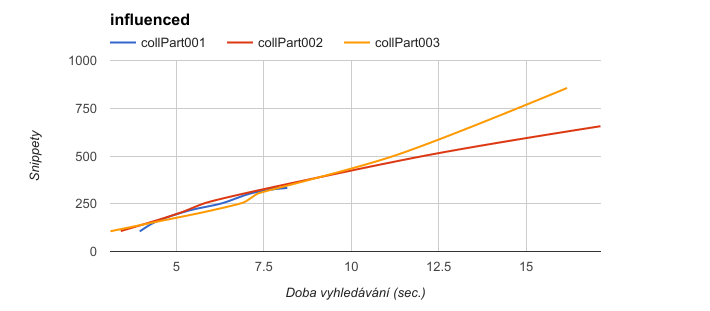
\includegraphics[scale=0.7]{obrazky-figures/influenced_time_n_of_snippets.png}
\caption{Graf závislosti mezi dobou vyhledávání a množstvím snippetů požadovaných k vyhledání pro dotaz \emph{influenced}. Graf byl sestrojen na základě tabulky \ref{influencedStats}}
\label{influenced_time_n_of_snpts}
\end{figure}

\begin{figure}[H]
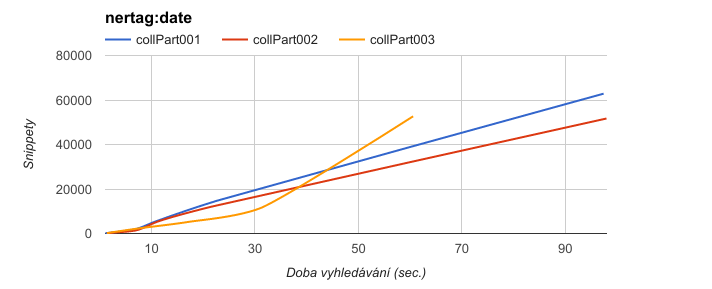
\includegraphics[scale=0.7]{obrazky-figures/nertag_date_time_n_of_snippets.png}
\caption{Graf závislosti mezi dobou vyhledávaní a množstvím snippetů požadovaných k vyhledání pro dotaz \emph{nertag:date}. Graf byl sestrojen na základě tabulky \ref{nertagdateStats}}
\label{nertag_date_time_n_of_snpts}
\end{figure}

\begin{figure}[H]
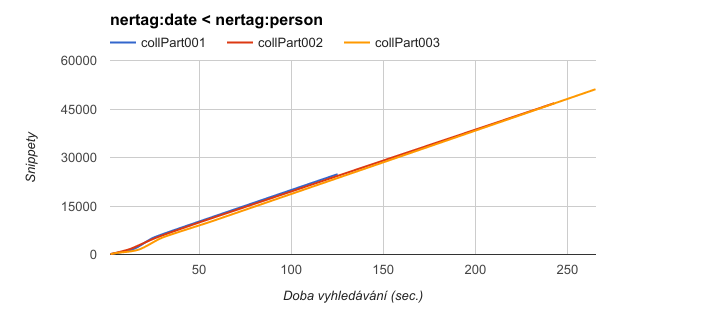
\includegraphics[scale=0.7]{obrazky-figures/nertag_date_nertag_person_time_n_of_snippets.png}
\caption{Graf závislosti mezi dobou vyhledávání a množstvím snippetů požadovaných k vyhledání pro dotaz \emph{nertag:date < nertag:person}. Graf byl sestrojen na základě tabulky \ref{nertagdatenertagpersonStats}}
\label{nertag_date_nertag_person_time_n_of_snpts}
\end{figure}

Třetím bodem je zjistit závislost doby  vyhledávání na složitosti dotazu. Pro odvození této závislosti byla použita tabulka  \ref{avgTime}. Na základě tabulky byl sestrojen graf \ref{time_complex}. Z~grafu vyplývá, že doba vyhledávání narůstá se složitostí dotazu. 

\begin{figure}[H]
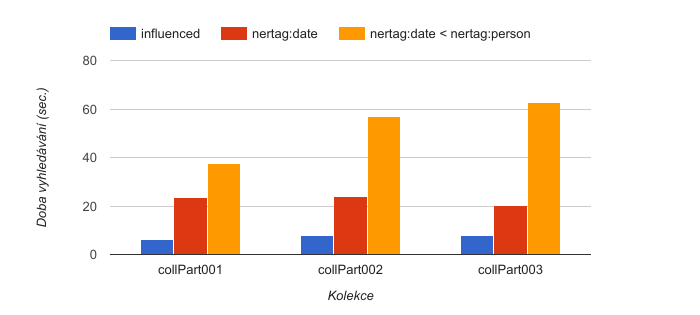
\includegraphics[scale=0.7]{obrazky-figures/time_complex.png}
\caption{Graf závislosti mezi dobou vyhledávání a složitostí dotazu}
\label{time_complex}
\end{figure}


Pro odvození vztahů z čtvrtého a pátého bodu byla  vytvořena  tabulka \ref{numbsStats}, ve které byli pro každý dotaz uvedené celkové množství snippetů, množství fragmentů v těchto snippetech a~množství dokumentů, ve kterých se tyto snippety vyskytly.  

\begin{table}[H]
\centering
\begin{tabular}{|c|c|c|c|}
\hline
\textbf{Dotaz} & \textbf{Snippety} & \textbf{Fragmenty} & \textbf{Dokumenty} \\
\hline
\emph{influenced} & 1844 & 1882 & 1600\\
\hline
\emph{nertag:date} & 358334 & 442381 & 83034 \\
\hline
\emph{nertag:date < nertag:person} & 131878 & 131878 & 49119 \\
\hline
\end{tabular}
\caption{Počet snippetů, fragmentů a dokumentů pro jednotlivé dotazy}
\label{numbsStats}
\end{table}


Pro odvození závislosti mezi počtem fragmentů a snippetů byla hodnota sloupce \textbf{Fragmenty} vydělena hodnotou sloupce \textbf{Snippety}:


\begin{itemize}
\item \emph{influenced}: $\frac{1882}{1844} \approx 1,021 $

\item \emph{nertag:person}: $\frac{442381}{358334} \approx 1,235$

\item \emph{nertag:date < nertag:person}: $\frac{131878}{131878} = 1$
\end{itemize}



Pro odvození závislosti mezi počtem dokumentů a množstvím fragmentů\,(snippetů) byla vydělená hodnota ze sloupce \textbf{Fragmenty}\,(\textbf{Snippety}) hodnotou ze sloupce \textbf{Dokumenty}:
\begin{itemize}
\item \emph{influenced}: $\frac{1882}{1600} \approx 1,176$ fragmentů v dokumentu; $\frac{1844}{1600} \approx 1,153$ snippetů v dokumentu

\item \emph{nertag:person}: $\frac{442381}{83034} \approx 5,328$ fragmentů v dokumentu; $\frac{358334}{83034} \approx 4,316$ snippetů v~dokumentu

\item \emph{nertag:date < nertag:person}: $\frac{131878}{49119} \approx 2,685$ fragmentů v dokumentu; $\frac{131878}{49119} \approx 2,685$ snippetů v dokumentu
\end{itemize}


\chapter{Závěr}
\label{chapter8}

Cílem této práce bylo navrhnout a implementovat software pro vyhledávání v sémanticky obohacených korpusech za použití rozsáhlých indexů MG4J na základě již existujícího řešení jako serverovou aplikaci, a také software pro komunikaci s více instancemi serverové části s~ohledem na~již existující webové rozhraní.

Zadání bylo splněno s dodržením všech klíčových bodů. Pro dotazování uživatel nemusí mít představu o struktuře souborů ve formátu mg4j, ale stačí mu základní povědomí o~jednotlivých doplňkových informacích, o entitách a ne-entitách. Uživatel definuje obsah fragmentů prostřednictvím dotazovacího jazyka MG4J-EQL. Překlad dotazu z jazyka MG4J-EQL na vyhledávací dotaz očekávaný nástrojem MG4J je řešen pomocí odpovídající třídy na straně serverové aplikace. Pro určení pracovních serverů slouží externí soubor, který je očekáván klientskou aplikací jako parametr při spouštění, nebo nastavení v konfiguračním souboru. Pro zajištění možnosti získat \uv{další dávku} dat slouží mechanizmus, který provádí serializaci adres serverů, které potenciálně mohou vrátit \uv{další dávku}, a serializaci posunů v rámci kolekcí jednotlivých serverů pro prevenci vrácení dat, která jíž byla vrácena v rámci předchozí komunikace. Možnost upřesňování dotazu prostřednictvím definice sémantických hodnot jednotlivých entit zajišťuje syntaxe jazyka MG4J-EQL. Pro obohacování entit\,(ne-entit) syntaktickými a sémantickými informacemi, které nejsou explicitně uvedeny v textu, má uživatel možnost definovat jednotlivé informace prostřednictvím konfiguračního souboru. Tento soubor slouží také pro definici pole, z jehož hodnot se výsledný text skládá. Pro zajištění kompatibility knihovny pro komunikaci se servery, společné pro webovou i textovou verzi klientské aplikace, byly požity jenom základní funkce jazyka \emph{Java}. Pro zvýraznění byly použity značky XML\,(HTML), které se mění na základě požadovaného stylu ASCII, RAW nebo HTML.

Na konci práce bylo provedeno testování vyvinutých částí systému. Testování bylo provedeno ve dvou fázích. Během první byla ověřena správnost jednotlivých částí. První fáze ukázala, že systém umí rozlišit mezi požadavkem na získání množiny snippetů a dokumentu a vrátit minimálně požadováné množství snippetů\,(v případě dostatku v kolekcích) či požadovaný dokument. Systém taktéž dokáže provádět patřičné zvýraznění podle stylu a~zcela validně provádět mapování mezi sémantickými hodnotami jednotlivých entit a sloupci v~souborech ve formátu mg4j. V~druhé fázi byly naměřeny hodnoty pro statistiky a určeny některé závislosti, které ukázaly, že doba vyhledání snippetů závisí jenom na množství vyhledávaných snippetů a složitosti dotazu, avšak nezávisí na velikosti kolekcí, ve kterých se vyhledávání provádí. Byly odvozeny i vztahy mezi množstvím snippetů, množstvím fragmentů a~množstvím dokumentů. 


Tuto práci považují za velmi užitečnou pro sebe, jako pro budoucího pracovníka v oblasti informačních technologií. Během výzkumu jsem nabyl nových znalostí z oblasti znalostních technologií, jako například výhody použití anotací, reprezentace sémantických dat, strukturu datově a dokumentově orientovaných systémů a další. Tuto práci považuji za důležitou i pro výzkumnou skupinu znalostních technologií. Předpokládá se, že vyvinutý systém bude v budoucnu používán studenty a pracovníky fakulty jako základ pro tvorbu dalších projektů, jako například analýza přirozeného jazyka s cílem odvození různých závislostí mezi entitami\,(jak jedna entita ovlivnila jinou apod.).


V budoucnu je možné práci rozšířit o zvýraznění nalezených fragmentů odpovídajících dotazu, implementaci post-podmínek, které by dovolily provádět pokročilejší filtrování výsledků, například vyhledat snippety, ve kterých se více než jedenkrát zmiňuje stejná entita, apod. K tomu lze využít strukturu \uv{\emph{snippets-parts-fields}}, která dovoluje jak implementaci post-podmínek, tak i zvýraznění. 


% Cílem této práce bylo navrhnout a implementovat software pro vyhledávání v sémanticky obohacených korpusech za použití rozsáhlých MG4J indexů na základě již existujícího řešení, jako serverové aplikace, a také software pro komunikaci se serverovými části s ohledem na již existující webové rozhraní.

% Zadání bylo splněno s dodržením všech klíčových bodů. Pro dotazování uživatel nemusí mít představu o struktuře souborů ve formátu mg4j, ale stačí mu základní povědomí o jednotlivých doplňkových informacích o entitách a ne-entitách. Uživatel definuje obsah fragmentů prostřednictvím dotazovacího jazyka MG4J-EQL. Překlad dotazu z jazyka MG4J-EQL na vyhledávací dotaz očekávaný nástrojem MG4J je řešen pomocí odpovídající třídy na straně serverové aplikace. Pro určení pracovních serverů slouží externí soubor, který je očekáván klientskou aplikaci jako parametr při spouštění, nebo nastavení v konfiguračním souboru. Při dotazování může uživatel definovat množství snippetů, které jsou požadovány od všech serverů, prostřednictvím parametru předaného aplikaci při spouštění. Každý server tedy obdrží požadavek na vyhledávání jenom části snippetů\,(očekávané množství snippetů od všech serverů se vydělí množstvím serverů). Pro zajištění možnosti získat další dávku dat, slouží mechanizmus, který provádí serializaci adres serverů, které potenciálně mohou vrátit další dávku, a serializaci posunů v rámci kolekcí jednotlivých serverů, pro prevenci vrácení dat, které jíž byli vráceny v rámci předchozí komunikace. V případě požadavku na získání další dávky se provádí deserializace. Možnost upřesňování dotazu prostřednictvím definice sémantických hodnot jednotlivých entit zajišťuje syntax jazyka MG4J-EQL. Pro rozšíření kontextů sémantickými a syntaktickými informacemi, které nejsou explicitně uvedeny v získané odpovědi, má uživatel možnost definovat jednotlivé informace prostřednictvím konfiguračního souboru. Tento soubor slouží také pro definici pole, z hodnot kterého se výsledný text skládá. Pro zajištění kompatibility knihovny pro komunikaci se servery, společné pro webovou i textovou verzi klientské aplikace, byli požity jenom základní funkce jazyka \emph{Java}. Pro zvýraznění byly použity tagy, známe z XML, které se mění na základě požadovaného stylu ASCII, RAW nebo HTML.

% Na konci práce bylo provedeno testování vyvinutých částí. Testování se provedlo ve dvou fázích. Během první byla ověřená správnost jednotlivých částí. První fáze ukázala, že systém umí rozlišit mezi požadavkem na získání množiny snippetů a dokumentu, a vrátit minimálně požadováné množství snippetů\,(v případě dostatku v kolekcích) a požadovaný dokument. Systém taktéž dokáže provádět patřičné zvýraznění podle stylu a zcela validně provádět mapování mezi sémantickými hodnotami jednotlivých entit a sloupci v mg4j souborech. V druhé fázi byli naměřené statistiky a odvozené některé závislosti, které ukázali, že doba vyhledání snippetů závisí jenom na množství vyhledávaných snippetů a složitosti dotazu, avšak zcela nezávisí na velikosti kolekcí, ve kterých se vyhledávání provádí. Byli odvozeny i vztahy mezi množstvím snippetů, množstvím fragmentů a množstvím dokumentů. 



% Tuto práci považují za velmi užitečnou pro sebe, jako pro budoucího pracovníka v oblasti informačních technologií. Během výzkumu jsem nabyl nových znalostí z oblasti znalostních technologií, jako například výhody použití anotací, reprezentaci sémantických dat, strukturu datově a dokumentově orientovaných systémů a další. 


% V budoucnu je možné práci rozšířit o zvýraznění nalezených fragmentů odpovídajících dotazu, implementaci post-podmínek, které by dovolili provádět více pokročile filtrování výsledků, například vyhledat snippety, ve kterých se více než jeden krát zmiňuje stejná entita apod. K tomu lze využít strukturu \uv{\emph{snippets-parts-fields}}, která dovoluje jak implementaci post-podmínek, tak i zvýraznění. 


























%=========================================================================
